\documentclass[a4paper, 12pt]{report}

\usepackage[dvipsnames]{xcolor}

%%%%%%%%%%%%%%%%
% Set Variables %
%%%%%%%%%%%%%%%%

\def\useItalian{0}  % 1 = Italian, 0 = English

\def\courseName{Computer Network Performance}

\def\coursePrerequisites{Networks and Probability}

\def\book{"Performance Modeling and Design of Computer Systems", M. Harchol-Balter}

\def\authorName{Simone Bianco}
\def\email{bianco.simone@outlook.it}
\def\github{https://github.com/Exyss/university-notes}
\def\linkedin{https://www.linkedin.com/in/simone-bianco}

% \def\authorName{Alessio Bandiera}
% \def\email{alessio.bandiera02@gmail.com}
% \def\github{https://github.com/aflaag-notes}
% \def\linkedin{https://www.linkedin.com/in/alessio-bandiera-a53767223}

%%%%%%%%%%%%
% Packages %
%%%%%%%%%%%%

\usepackage{../../packages/Nyx/nyx-packages}
\usepackage{../../packages/Nyx/nyx-styles}
\usepackage{../../packages/Nyx/nyx-frames}
\usepackage{../../packages/Nyx/nyx-macros}
\usepackage{../../packages/Nyx/nyx-title}
\usepackage{../../packages/Nyx/nyx-intro}

%%%%%%%%%%%%%%
% Title-page %
%%%%%%%%%%%%%%

\logo{../../packages/Nyx/logo.png}

\if\useItalian1
    \institute{\curlyquotes{\hspace{0.25mm}Sapienza} Università di Roma}
    \faculty{Ingegneria dell'Informazione,\\Informatica e Statistica}
    \department{Dipartimento di Informatica}
    \ifdefined\book
        \subtitle{Appunti integrati con il libro \book}
    \fi
    \author{\textit{Autore}\\\authorName}
\else
    \institute{\curlyquotes{\hspace{0.25mm}Sapienza} University of Rome}
    \faculty{Faculty of Information Engineering,\\Informatics and Statistics}
    \department{Department of Computer Science}
    \ifdefined\book
        \subtitle{Lecture notes integrated with the book \book}
    \fi
    \author{\textit{Author}\\\authorName}
\fi


\title{\courseName}
\date{\today}

% \supervisor{Linus \textsc{Torvalds}}
% \context{Well, I was bored\ldots}

\usetikzlibrary{chains,shapes.multipart}
\usetikzlibrary{shapes,calc,fit}
\usetikzlibrary{automata,positioning,shapes.multipart}

\newcounter{cntr}
\tikzset{
    queue/.style={scale=0.8,inner sep=1pt,draw,rectangle split,rectangle split horizontal,minimum height=1.25cm,rectangle split parts=5, draw, xshift=-10, font=\sffamily\normalsize},
}

%%%%%%%%%%%%
% Document %
%%%%%%%%%%%%

\begin{document}
    \maketitle

    % The following style changes are valid only inside this scope 
    {
        \hypersetup{allcolors=black}
        \fancypagestyle{plain}{%
        \fancyhead{}        % clear all header fields
        \fancyfoot{}        % clear all header fields
        \fancyfoot[C]{\thepage}
        \renewcommand{\headrulewidth}{0pt}
        \renewcommand{\footrulewidth}{0pt}}

        \romantableofcontents
    }

    \introduction

    %%%%%%%%%%%%%%%%%%%%%

    \chapter{Queueing theory}

    \section{Introduction to performance evaluation}

    The modern digital infrastructure is based on networks formed of hundres of interconnected computer systems. To manage the ingoing and outgoing traffic, \textit{queuing} is essential. \textbf{Queueing theory} is the study of what happens when many \textit{jobs} compete for limited resources, often resulting in queues and delays due to the system not being capable of serving every incoming job at once. At its core, this theory seeks to explain why queues form, how they behave and what can be done to minimize or eliminate them.

    Consider a simple example: a computer system, such as a web server, handling just one job. The job arrives, consumes some resources (like CPU and I/O), and then departs. Since there are no other jobs in the system, it's easy to predict exactly when it will finish: there's no waiting time and no queue. However, resources are often shared among many jobs, leading to contention and delays.
    
    The first goal of queueing theory is \textbf{predicting} the system's performances that we're interested in. The second goal is to \textbf{improve design} in order to achieve a better performance. We'll start by giving some concrete examples of performance prediction and system analysis. First, we'll give some definitions.
    
    \begin{frameddefn}{Open and closed system}
        A system is said to be open if there is at at least one way for jobs to exit the system. If no way exists, the system is said to be closed. 
    \end{frameddefn}
    
    \begin{figure}[H]
        \centering

            \begin{tabular}{ccc}
                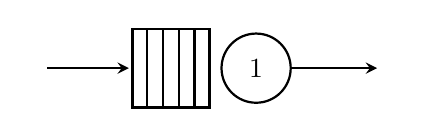
\begin{tikzpicture}[->,>=stealth,shorten >=1pt,auto,node distance=1cm,thick,main node/.style={scale=0.8,circle,draw,font=\sffamily\normalsize}]
                \node[state] (s1) []{$1$};
                \node[queue] (b1) [left of = s1]{};
                \node[] (l1) [left of = b1, xshift=-20]{};
                \node[] (x1) [right of = s1, xshift=20]{};

                \path[every node/.style={font=\sffamily\small}]
                    (l1) edge (b1.west)
                    (s1.east) edge (x1)
                    ;
            \end{tikzpicture}

            &\qquad\qquad&

            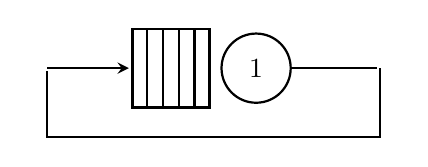
\begin{tikzpicture}[->,>=stealth,shorten >=1pt,auto,node distance=1cm,thick,main node/.style={scale=0.8,circle,draw,font=\sffamily\normalsize}]
                \node[state] (s1) []{$1$};
                \node[queue] (b1) [left of = s1]{};
                \node[] (l1) [left of = b1, xshift=-20]{};
                \node[] (x1) [right of = s1, xshift=20]{};

                \path[every node/.style={font=\sffamily\small}]
                    (l1) edge (b1.west)
                    (s1.east) [-]edge (x1)
                    ;

                \draw[-] (x1.west) -- +(0, -25pt) -- ($(l1.east)+(0, -25pt)$) -- (l1.east);
            \end{tikzpicture}
        \end{tabular}

        \caption{An open system and a closed system, both with one server and its queue.}
    \end{figure}

    We observe that closed systems may or may not contain a \curlyquotes{thinking center}, i.e. a subsystem of terminals that does some work before sending jobs to the system. Closed systems that don't contain such thinking center are called \textit{batch systems}, while the others are called \textit{interactive systems}.

    \begin{figure}[H]
        \centering
        \includegraphics[scale=0.75]{images/batch_interactive.png}
        \caption{A batch system (left) and an interactive system (right)}
    \end{figure}

    In order to analyze and predict the behavior of a queueing system, we must first define a few key performance metrics. These metrics describe how jobs arrive, how quickly they are served and how efficiently the system operates overall. We start by defining three main parameters.

    The \textbf{arrival rate}, typically denoted by $\lambda$ and measured in jobs per unit of time, represents how frequently new jobs enter the system. For example, if an average of 10 jobs arrive every second, then $\lambda = 10$ jobs/second. In most queueing models, job arrivals are assumed to follow a random process -- often a Poisson process -- meaning that the times between successive arrivals are independent and exponentially distributed. The arrival rate thus characterizes the workload intensity imposed on the system.

    The \textbf{service rate}, typically denoted by $\mu$, measures how quickly the system can process jobs. Specifically, it represents the average number of jobs that can be completed per unit of time by a single server. For instance, if a server can complete 5 jobs per second on average, then $\mu = 5$ jobs/second.

    The \textbf{throughput}, typically denoted by $X$, indicates the actual rate at which jobs are completed and leave the system. If a server processes 6 jobs per second on average, then $X = 6$ jobs/second. 

    \begin{figure}[H]
        \centering

        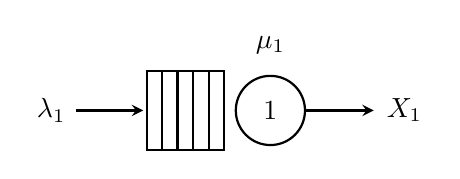
\begin{tikzpicture}[->,>=stealth,shorten >=1pt,auto,node distance=1cm,thick,main node/.style={scale=0.8,circle,draw,font=\sffamily\normalsize}]
        \node[state] (s1) []{$1$};
        \node[queue] (b1) [left of = s1]{};
        \node[] (l1) [left of = b1, xshift=-20]{$\lambda_1$};
        \node[] (m1) [above of = s1, yshift=-5]{$\mu_1$};
        \node[] (x1) [right of = s1, xshift=20]{$X_1$};

        \path[every node/.style={font=\sffamily\small}]
            (l1) edge (b1.west)
            (s1.east) edge (x1)
            ;
        \end{tikzpicture}

        \caption{A device and its parameters.}
    \end{figure}

    To formally define these three metrics, we introduce three \textbf{elementary measures} based on elapsed time. Given a time instant $t$ and a device $i$, let:
    \begin{enumerate}
        \item $A_i(t)$ denote the total number of jobs arrived at device $i$ at time $t$
        \item $C_i(t)$ denote the total number of jobs completed by device $i$ at time $t$
        \item $B_i(t)$ denote the total number of seconds the device $i$ was busy working on jobs at time $t$
    \end{enumerate}

    For the arrival rate and the throughput, we can express there two metrics as the ratio between the number of jobs of interest over the total amount of time $t$ that elapsed (as $t \to +\infty$).

    \begin{frameddefn}{Arrival rate and Throughput}
        Given a device $i$, we define the arrival rate $\lambda_i$ and the throughput $X_i$ of device $i$ as:
        \[\lambda_i = \lim_{t \to +\infty} \frac{A_i(t)}{t} \qquad\qquad X_i = \lim_{t \to +\infty} \frac{C_i(t)}{t}\] 
    \end{frameddefn}
    
    For the service rate, instead, we must restrict our interest only to the portion of time for which the device was actually busy working (otherwise, we would also be accounting for the time spent by jobs waiting in the queue).

    \begin{frameddefn}{Service rate}
        Given a device $i$, we define the service rate $\mu_i$ of device $i$ as:
        \[\mu_i = \lim_{t \to +\infty} \frac{C_i(t)}{B_i(t)}\]
    \end{frameddefn}

    These three fundamental measures can also be defined at \textbf{global} level, i.e. for the whole system. In this case, they are usually denoted with $\lambda, \mu, X$ and they are defined as: 
    \[\lambda = \lim_{t \to +\infty} \frac{A(t)}{t} \qquad \mu = \lim_{t \to +\infty} \frac{C(t)}{B(t)} \qquad X = \lim_{t \to +\infty} \frac{C(t)}{t}\] 

    where $A(t)$ and $C(t)$ are the total number of arrived and completed jobs in the system, while $B(t)$ is the total number of seconds that the system was busy working (i.e. with at least one device working). From now on, we'll always assume that the symbols $\lambda, \mu$ and $X$ refer to these three parameters. When we have a system with multiple servers, we'll use pedices to distinguish the servers' parameters (e.g. $\lambda_1, \mu_1, X_1$ are the parameters of Server 1). When the subscript is omitted, we're usually referring to the global metric, i.e. the metric over the whole system.

    \section{System stability}
    
    In order for performance measures to actually mean something, the system must be working at full capacity (hence why we consider $t \to +\infty$). When the system is closed, this hypothesis is not required since even a single job is able to make the system always operational (no idle time). We observe that these three parameters are strictly related to each other and may act as a bottleneck:
    \begin{itemize}
        \item If $\lambda < \mu$, the system receives at most as many jobs than those that it can process, meaning that it is able to serve them all. Hence, we get that $X = \lambda$.
        \item If $\lambda \geq \mu$, the system receives more jobs than those that it can process, meaning that it will be forced to drop some of them. Hence, we get that $X = \mu$.
    \end{itemize}

    We observe that the relationship between the arrival rate and the service rate not only defines the value of the throughput, but it also defined the \textbf{stability} of the system. A system is said to be \textit{stable} when there is no queue build-up any device of the system, i.e. the size of every queue of each device doesn't \curlyquotes{explode}, becoming too large (thus forcing the devices to drop incoming jobs). It's easy to see that a system is stable if and only if each device is able to process jobs faster than they arrive in the queue, meaning that $\lambda_i < \mu_i$.

    \begin{framedprop}{System stability}
        A system is stable if and only if for every device $i$ it holds that $\lambda_i \leq \mu_i$.
    \end{framedprop}

    \begin{proof}
        We prove both directions. First, it's easy to see that if $\lambda_i \leq \mu_i$ holds for every $i$ then each device is able to process every incoming job without queue build-up, concluding that the system is stable.

        Let $A_i^{\text{queue}}(t)$ and $D_i^{\text{queue}}(t)$ respectively denote the number of jobs arrived to and departed from the queue of device $i$ up to time $t$. Similarly, let $N_i^{\text{queue}}(t)$ be the number of jobs in the queue of device $i$ at time $t$. We observe that:
        \[N_i^{\text{queue}}(t) = A_i^{\text{queue}}(t) - D_i^{\text{queue}}(t)\]

        By definition, we have that $A_i^{\text{queue}}(t) = A_i(t) = \lambda t$. Similarly, we have that $D_i^{\text{queue}}(t) \leq \mu t$ (due to the fact that some jobs may be dropped due to the queue being full). This implies that:
        \[N_i^{\text{queue}}(t) = A_i^{\text{queue}}(t) - D_i^{\text{queue}}(t) \geq \lambda t - \mu t = (\lambda - \mu) t\]

        By contrapositive, suppose that there is at least one device $j$ such that $\lambda_j > \mu_j$. Then, as $t \to +\infty$ we get that $N_j^{\text{queue}}(t) = +\infty$, meaning that the system is unstable.
    \end{proof}

    Clearly, we want to restrict our interest to systems that are stable since measuring the performance of an unstable system has no real use (every measure either goes to infinity or to zero as time elapses). Hence, from now on we'll \underline{assume to be working with stable systems}. Since $\lambda_i = \mu_i$ holds for every device in stable systems, we know that the throughput is limited by the arrival rate, thus $X_i = \lambda_i < \mu_i$. In closed systems, the equality $X_i = \lambda_i$ always holds (even in unstable conditions) due to necessary packet drops.

    \begin{framedprop}{}
        Given a device $i$, it holds that:
        \begin{itemize}
            \item If the system is closed then $X_i = \lambda_i$
            \item If the system is open then $X_i = \lambda_i$ if and only if the system is stable
        \end{itemize}
    \end{framedprop}

    Each time we want to change some part of the system, we have to ensure that stability is preserved. For instance, consider the following system with probabilistic routing.

    \begin{figure}[H]
        \centering
        \includegraphics[scale=0.6]{images/prob_queueing.png}
        \caption{A system with probabilistic routing}
    \end{figure}

    Here, each device $i$ receives external arrivals with rate $r_i$, but it also receives internal arrivals from some of the other servers. The sum of these two arrival rates corresponds to the total arrival rate $\lambda_i$. Each packet that is processed by device $i$ is next routed to server $j$ with probability $p_{i,j}$, where the device \curlyquotes{out} represents the outside of the system.

    Suppose that $\mu_1 = \mu_2 = \mu_3 = 10$ j/s (jobs/seconds) and that $r_2 = r_3 = 1$ j/s. The routing probabilities are set to the following values:
    \begin{itemize}
        \item $p_{1,2} = p_{2,out} = 0.8$
        \item $p_{2,3} = p_{1,3} = 0.2$
        \item $p_{3,1} = 1$
    \end{itemize}

    We want to find the maximum possible value for the external arrival rate $r_1$, preserving stability. First, we observe that:
    \[\soe{ll}{
        \lambda_1 = r_1 + p_{3,1} X_3 \\
        \lambda_2 = r_2 + p_{1,2} X_1 \\
        \lambda_3 = r_3 + p_{1,3} X_1 + p_{2,3} X_2 \\
    }\]

    Since we want stability to hold, we can assme that $X_i = \lambda_i$ holds for each device $i$. Substituting the probabilities, we obtain that:
    \[\soe{ll}{
        \lambda_1 = r_1 + \lambda_3 \\
        \lambda_2 = r_2 + \frac{8}{10}\lambda_1 \\
        \lambda_3 = r_3 + \frac{2}{10}\lambda_1 + p_{2,3} \lambda_2 \\
    }\]

    Solving the system in function of $r_1$, we obtain that:
    \[\soe{ll}{
        \lambda_1 = \frac{15}{8} + \frac{25}{16} r_1\\
        \lambda_2 = \frac{5}{4} + \frac{5}{4} r_1\\
        \lambda_3 = \frac{15}{8} + \frac{9}{16} r_1\\
    }\]

    To impose stability, we know that $\lambda_i < \mu_i$ must hold for every device $i$. Therefore, we get that:
    \[\soe{ll}{
        10 > \frac{15}{8} + \frac{25}{16} r_1\\
        10 > \frac{5}{4} + \frac{5}{4} r_1\\
        10 > \frac{15}{8} + \frac{9}{16} r_1\\
    }\]

    Solving each inequality, we conclude that:
    \[\soe{ll}{
        r_1 < \frac{26}{5} \\
        r_1 < 6 \\
        r_1 < \frac{130}{9}
    }\]

    Thus, in order for the system to be stable the value of $r_1$ must be such that:
    \[r_1 < \min \rbk{\frac{26}{5}, 6, \frac{130}{9}} = \frac{26}{5}\]

    \section{Utilization and time analysis}

    In the previous sections introduced rate metrics to analyze the speed of the system. But what about time metrics? In particular, we're interested in knowing performances such as how much is a device working, the time required by a job to be processed by the whole system and by a single device.

    The first metric that we're going to introduce is the \textbf{utilization} of a device, written as $\rho_i$, which describes how busy a device is. Intuitively, this metric is represented as the ratio between the the time in which the device was busy working over the total elapsed time.

    \begin{frameddefn}{Utilization}
        Given a device $i$, we define the utilization $\rho_i$ as:
        \[\rho_i = \lim_{t \to +\infty}\frac{B_i(t)}{t}\]
    \end{frameddefn}

    Since the utilization is described as the percentage of time the device was busy working, it's easy to see that:
    \[\begin{split}
        \rho_i &= \Pr[\text{device $i$ is busy}] \\
        &= \Pr[N^{\text{server}}_i = 1] \\
        &= 1 \cdot \Pr[N^{\text{server}}_i = 1] + 0 \cdot \Pr[N^{\text{server}}_i = 0] \\
        &= \Exp[N^{\text{server}}_i]
    \end{split}\]

    where $N^{\text{server}}_i$ is the \textbf{server population} of device $i$, that being the number of jobs in the server of device $i$ (thus not in the queue), which is at most 1.

    The second metric that we're going to introduce is \textbf{service time}, typically written as $S_i$. Intuitively, this is the time spent by a device to process a job. By definition, the average service time of a device is nothing more than the inverse of its service rate.

    \begin{frameddefn}{Service time}
        Given a device $i$, we define the service time $S_i$ of device $i$ as the random variable such that:
        \[\Exp[S_i] = \frac{1}{\mu_i}\]
    \end{frameddefn}

    Clearly, the above definition implies that:
    \[\Exp[S_i] = \frac{1}{\mu_i} = \lim_{t \to +\infty} \frac{B_i(t)}{C_i(t)}\]

    This allows us to formalize our first law, known as the \textbf{utilization law}.

    \begin{framedlaw}{Utilization law}
        Given a device $i$, it holds that:
        \[\rho_i = \Exp[S_i] X_i\]
    \end{framedlaw}

    \begin{proof}[Proof through definitions]
        Through easy algebraic manipulation we get that:
        \[X_i = \frac{C_i(\tau)}{\tau} = \frac{C_i(\tau)}{B_i(\tau)} \cdot \frac{B_i(\tau)}{\tau} = \mu_i \rho_i\]

        Thus, we conclude that $\rho_i = \Exp[S_i] X_i$.
    \end{proof}

    \begin{proof}[Proof through expected value]
        By definition, we have that:
        \[\begin{split}
            X_i &= \Exp[\text{Completion rate of $i$}] \\
            &= \Exp[\text{Completion rate of $i$} \mid \text{$i$ is busy}] \Pr[\text{$i$ is busy}] \\
            &\quad + \Exp[\text{Completion rate of $i$} \mid \text{$i$ isn't busy}] \Pr[\text{$i$ isn't busy}] \\
            &= \mu_i \rho_i + 0 (1-\rho_i) \\
            &= \mu_i \rho_i
        \end{split}\]

        Thus, we conclude that $\rho_i = \Exp[S_i] X_i$.
    \end{proof}

    To avoid confusion, we remark that service time referes \underline{only} to the time spent by the job inside the device itself, thus without considering the time spent by it inside its queue. This latter metric is known as \textbf{waiting time}, written as $W_i$. When considering both portion sof time, the metric is known as \textbf{response time}, the time spent by a single job be fully served by a device.

    \begin{frameddefn}{Response time}
        Given a device $i$, we define the response time $R_i$ of device $i$ as the random variable such that:
        \[\Exp[R_i] = \Exp[W_i] + \Exp[S_i]\]
        where $W_i$ is the time spent by a job inside the queue of device $i$.
    \end{frameddefn}

    Consider a single device $i$. When the system is stable, we know that jobs are being processed faster than their arrival in the queue ($\mu_i > \lambda_i$). In this case, the value $\mu_i - \lambda_i$ represents how much faster the server can serve customers than they arrive, namely the \textit{net service capacity}. It's easy to see that the inverse of such metric is exactly the average response time of the device.
    
    \begin{framedprop}{}
        Consider a stable system. Given a device $i$, it holds that:
        \[\Exp[R_i] = \frac{1}{\mu_i - \lambda_i}\]
    \end{framedprop}

    Through the above result, we also conclude that:
    \[\Exp[W_i] = \Exp[R_i] - \Exp[S_i] = \frac{1}{\mu_i - \lambda_i} - \frac{1}{\mu_i}= \frac{\lambda_i}{\mu_i(\mu_i - \lambda_i)}\]

    Since $X_i = \lambda_i$ holds, through the utilization law, we conclude that:
    \[\Exp[W_i] = \frac{\lambda_i}{\mu_i(\mu_i - \lambda_i)} = \frac{X_i}{\mu_i(\mu_i - \lambda_i)} = \rho \Exp[R_i]\]

    In other words, the average time spend by a time in the queue is given by the average time required by a job to be fully processed by the device and the workload of the device itself.

    \newpage

    \section{Little's law}

    We introduce two new global metrics: the system traversal time and the system response time. The \textbf{system traversal time} can be informally described as the time required by a job to go from \curlyquotes{out} of the system to \curlyquotes{out} of the system. The \textbf{system response time}, instead, can be informally described as the time required by a job to go from \curlyquotes{into} the system to \curlyquotes{out} of the system.
    
    For open systems, it holds that $\Exp[T] = \Exp[R]$ since there is no difference from coming out of the system or into the system due to all jobs coming from the outside. For closed system, instead, the traversal time may also contain time required by the system to \curlyquotes{think} (e.g. we're working with an interactive system). Thus, we have that $\Exp[T] = \Exp[R] + \Exp[Z]$, where $Z$ is the \textbf{thinking time} of the system. If the closed system has no thinking center, we can simply set $\Exp[Z] = 0$.

    \begin{frameddefn}{Traversal time}
        The traversal time $T$ of a system is the random variable such that:
        \begin{itemize}
            \item $\Exp[T] = \Exp[R]$ if the system is open
            \item $\Exp[T] = \Exp[R] + \Exp[Z]$ if the system is closed
        \end{itemize}
    \end{frameddefn}

    To compute the value of $\Exp[R]$, we usually use Little's Law, one of the most powerful and elegant results in queueing theory and operations management. It provides a simple relationship between three fundamental performance measures of any stable system. Formally, it states that $\Exp[T] = \frac{\Exp[N]}{X}$, where $N$ is the number of jobs in the system. In order for such law to hold, the system must be \textbf{ergodic}.

    \begin{frameddefn}{Ergodic system}
        A system is said to be ergodic if it has the following three properties:
        \begin{itemize}
            \item \textit{Irreducibility}: from every state (defined as the population in the servers) the system can reach every other state and back.
            \item \textit{Positive recurrence}: starting from a state, the probability to return in that same state over infinite time is 1.
            \item \textit{Aperiodicity}: the system doesn't have a periodic behavior, meaning that it doesn't return in a specific state after a precise amount of time.
        \end{itemize}
    \end{frameddefn}

    \begin{framedlaw}[label={little}]{Little's law}
        Given an ergodic system, it holds that:
        \[\Exp[T] = \frac{\Exp[N]}{X}\]
    \end{framedlaw}

    \begin{proof}
        Fix a generic time instant $t$. Let $\mathcal{A}(t)$ denote the area used by the jobs up to time $t$ (see figure \Cref{little_law}). Interpreting the graph as a continuous function, we get that:
        \[\mathcal{A}(t) = \int_{0}^{t} N(s) \, ds\]

        where $N(s)$ denotes the number of jobs in the system at time $s$. For each job $j$, let $T_j$ denote the time required to complete job $j$. Moreover, let $J_A(t), J_C(t)$ denote, respectively, the set of arrived and completed jobs at time $t$. We observe that:
        \[\sum_{j \in J_C(t)} T_j \leq \mathcal{A}(t) \leq \sum_{j \in J_A(t)} T_j\]

        Dividing  the whole inequality by $t$ we get that:
        \[\frac{1}{t} \sum_{j \in J_C(t)} T_j \leq \frac{1}{t} \int_{0}^{t} N(s) \, ds \leq \frac{1}{t} \sum_{j \in J_A(t)} T_j\]

        Through algebraic manipulation we get that:
        \[\frac{C(t)}{t} \cdot \frac{\sum_{j \in J_C(t)} T_j}{C(t)} \leq \frac{\int_{0}^{t} N(s) \, ds}{t} \leq \frac{A(t)}{t} \cdot \frac{\sum_{j \in J_A(t)} T_j}{A(t)}\]

        By taking the limit as $t \to +\infty$, we obtain that:
        \[\begin{split}
            & \lim_{t \to +\infty} \frac{C(t)}{t} \cdot \frac{\sum_{j \in J_C(t)} T_j}{C(t)} \leq \lim_{t \to +\infty} \frac{\int_{0}^{t} N(s) \, ds}{t} \leq \lim_{t \to +\infty} \frac{A(t)}{t} \cdot \frac{\sum_{j \in J_A(t)} T_j}{A(t)} \\
            \implies & X \cdot \lim_{t \to +\infty} \frac{\sum_{j \in J_C(t)} T_j}{C(t)} \leq \Exp[N] \leq X \cdot \lim_{t \to +\infty} \frac{\sum_{j \in J_A(t)} T_j}{A(t)}
        \end{split}\]

        since $\lim_{t \to +\infty} \frac{C(t)}{t} = X$ and $\lim_{t \to +\infty} \frac{A(t)}{t} = \lambda = X$. Moreover, we observe that as $t \to +\infty$ the difference between arrival and completion becomes negligible. Thus, we get that:
        \[\lim_{t \to +\infty} \frac{\sum_{j \in J_C(t)} T_j}{C(t)} = \Exp[T] = \lim_{t \to +\infty} \frac{\sum_{j \in J_A(t)} T_j}{A(t)}\]

        concluding that $X \Exp[T] \leq \Exp[N] \leq X \Exp[T]$.
    \end{proof}

    \begin{figure}[H]
        \centering
        \includegraphics[scale=0.65]{images/ll_open.png}
        \includegraphics[scale=0.65]{images/ll_closed.png}

        \caption{Graph of job system times in open system (above) and closed systems (below). The darker area corresponds to $\mathcal{A}(t)$.}
        \label{little_law}
    \end{figure}

    After proving the law's correctness, we discuss its applications. First of all, we observe that the law can be made more explicit for open and closed systems by expanding the traversal time. For open systems we have that:
    \[\Exp[R] = \Exp[T] = \frac{\Exp[N]}{X}\]

    For closed systems, we also observe that $\Exp[N] = N$ since the number of jobs in the system is constant. Thus:
    \[\Exp[R] = \frac{N}{X} - \Exp[Z]\]

    The latter formula is also known as \textbf{response time law for closed systems}.
    
    Nonetheless, the true power of the law comes from the fact that it can be applied not only to the whole system but also to \underline{sub-systems}.
    The key idea here is that any sub-system can be viewed as a \curlyquotes{box} with ingoing and outgoing jobs. Then, each box can be viewed as an open system on which the law can be applied.

    For instance, consider the following interactive system with a central system deployed in the cloud (thus we don't know its interal connections).
    
    \begin{figure}[H]
        \centering
        \includegraphics[scale=0.55]{images/ll_ex0.png}

        \caption{An interactive system with a cloud central system}
    \end{figure}

    The following information about the system is known:
    \begin{itemize}
        \item $\Exp[N] = 23$
        \item $\Exp[Z] = 21$ secs
        \item $X = 0.45$ jobs/secs
        \item $\Exp[N_{\text{mem}}] = 11.65$
    \end{itemize}
    
    We want to compute the response time of the central cloud system, namely $R_{\text{cloud}}$. With the known information, we can easily apply the response time law to the whole system, obtaining that:
    \[\Exp[T] = \frac{\Exp[N]}{X} - \Exp[Z] = 23 \cdot \frac{100}{45} - 21 = \frac{271}{9} \text{ sec}\]

    Now, we use the real power of Little's law. Consider the following sub-system described by the red box. We refer to this sub-system as \textit{mem-sys}.

    \begin{figure}[H]
        \centering
        \includegraphics[scale=0.4]{images/ll_ex0_2.png}

        \caption{The mem-sys sub-system.}
    \end{figure}

    Similarly, the cloud center can also be viewed as a sub-system. We observe that
    \[\Exp[R_{\text{cloud}}] = \Exp[T] - \Exp[R_{\text{mem-sys}}]\]

    Since this mem-sys sub-system can be viewed as an open system, by Little's law we have that:
    \[\Exp[R_{\text{mem-sys}}] = \frac{\Exp[N_{\text{mem-sys}}]}{X_{\text{mem-sys}}}\]

    Now, we observe that $X_{\text{mem-sys}} = X$ since every job of the system enters to and exits from mem-sys. Moreover, we also have that $\Exp[N_{\text{mem-sys}}] = \Exp[N_{\text{mem}}]$, concluding that:
    \[\Exp[R_{\text{mem-sys}}] = \frac{\Exp[N_{\text{mem-sys}}]}{X_{\text{mem-sys}}}= \frac{\Exp[N_{\text{mem}}]}{X} = \frac{1165}{100} \frac{100}{45} = \frac{233}{9} \text{ sec}\]

    Therefore, we conclude that:
    \[\Exp[R_{\text{cloud}}] = \Exp[T] - \Exp[R_{\text{mem-sys}}] = \frac{271}{9} -  \frac{233}{9} = \frac{38}{9}\]

    On a simpler case, Little's law can also be used to derive the utilization law. Given a system made of a single device, we can consider the sub-system composed only by the server. Since there is no queue in the system, we know that $\Exp[R_i^{\text{server}}] = \Exp[S_i^{\text{server}}]$. Then, byLittle's law we conclude that:
    \[\Exp[S_i^{\text{server}}] = \Exp[R_i^{\text{server}}] = \frac{\Exp[N_i^{\text{server}}]}{X_i^{\text{server}}} = \frac{\rho}{X_i}\]

    \begin{figure}[H]
        \centering
        \includegraphics[scale=0.8]{images/util_ll.png}

        \caption{The sub-system considered to derive the utilization law}
    \end{figure}

    \section{Forced flow law}

    Consider the following interactive system with a CPU device. The device has two outgoing links: one that goes back to the terminal center and one that loops back into the device itself. Each job exiting the device has $\frac{1}{2}$ probability of looping back and $\frac{1}{2}$ probability of going back to the terminal.

    \begin{figure}[H]
        \centering
        \includegraphics[scale=0.7]{images/ll_ex1.png}

        \caption{An interactive system with a fork with $0.5$ probability of going back to the terminals.}
    \end{figure}

    Consider now the sub-system formed of the CPU device and the looping link (represented by the red box in \Cref{ll_ex1_2}). Since every job of the system enters and exits from this sub-system, we know that the throughput of the latter must be equal to the system throughput. Thus, we have that $X_{\text{sub-sys}} = X$.
    
    But what about the throughput of the sub-system formed only by the CPU device (represented by the green box in \Cref{ll_ex1_2})? We notice that every job that exits the CPU and goes back to the terminal center gets accounted both for the CPU throughput and the global system throughput. Since each exiting job has $\frac{1}{2}$ probability of going back to the terminal center, we can expect that $X = \frac{1}{2}X_i$. Indeed, this is the case!
    
    \begin{figure}[H]
        \centering
        \includegraphics[scale=0.5]{images/ll_ex1_2.png}

        \caption{The two sub-systems.}
        \label{ll_ex1_2}
    \end{figure}

    In general, the relationship between the overall system throughput and the throughput of each individual service center within the system is described by the \textbf{forced flow law}, which formally states that $X_i = \Exp[V_i] X$. Here, $V_i$ is the \textbf{visit ratio} of the device, that being the number of visits any job makes to the device.
    
    \begin{frameddefn}{Visit ratio}
        Given a device $i$, we define the visit ratio $S_i$ of device $i$ as:
        \[V_i = \lim_{t \to +\infty} \frac{C_i(t)}{C(t)}\]
    \end{frameddefn}

    \begin{framedlaw}{Forced flow law}
        Given a device $i$, it holds that:
        \[X_i = \Exp[V_i] X\]
    \end{framedlaw}

    \begin{proof}
        Let $V_i^{(j)}$ be the number of visits that the $j$-th job makes to device $i$. Let $J_C(t)$ be the set of completed jobs at time $t$. We observe that:
        \[C_i(t) = \sum_{j \in J_C(t)} V_i^{(j)}\]

        Dividing the whole equality by $t$ and rewriting the right-hand side, we get that:
        \[\frac{C_i(t)}{t} = \frac{\sum_{j \in J_C(t)} V_i^{(j)}}{t} = \frac{\sum_{j \in J_C(t)} V_i^{(j)}}{C(t)} \cdot \frac{C(t)}{t}\]

        By taking the limit as $t \to +\infty$, we obtain that:
        \[\begin{split}
            \lim_{t \to +\infty} \frac{C_i(t)}{t} = \lim_{t \to +\infty} \frac{\sum_{j \in J_C(t)} V_i^{(j)}}{C(t)} \cdot \frac{C(t)}{t} \implies X_i = \Exp[V_i] X
        \end{split}\]
    \end{proof}

    Computing the value of $\Exp[V_i]$ is not an easy task since it highly depends on the structure of the system and the probabilities of each link. For instance, consider the following generalization of the previous example.

    \begin{figure}[H]
        \centering
        \includegraphics[scale=0.5]{images/forc_flow.png}

        \caption{An interactive system with a fork with $p$ probability of going back to the terminals.}
    \end{figure}

    First of all, we observe that $\Pr[V_i = k] = \Pr[\text{the job exits after looping $k-1$ times}]$ since one visit is accounted when the job exits the loop. Moreover, probabilistically speaking, it is possible for a job to loop indefinitely in the system. Thus, we have that:
    \[\Exp[V_i] = \sum_{k = 0}^{+\infty} k \Pr[V_i = k] = \sum_{k = 0}^{+\infty} k \Pr[\text{the job exits after looping $k-1$ times}]\]

    Now, it's easy to see that the event of looping $k-1$ times inside the device is described by a geometric process: in order to exit at the $k$-th iteration, the job must first loop for $k-1$ times, meaning that:
    \[\Pr[\text{the job exits after looping $k-1$ times}] = (1-p)^{k-1}p\]

    Thus, we get that:
    \[\Exp[V_i] = \sum_{k = 0}^{+\infty} k (1-p)^k p\]

    concluding that $V_i$ is an r.v. with geometric distribution of parameter $p$. Identifying the distribution type of $V_i$ allows us to immediately compute its expected value through known results. In particular, since $V_i \sim \mathrm{Geo}(p)$, we immediately get that $\Exp[V_i] = \frac{1}{p}$. In other words, the averagae number of visits received by device $i$ is the inverse of the probability of a job exiting the loop. Going back to our original example, we get that $X_i = 2 X$ as expected by our observation.

    The forced flow law also gives us an additional way to express the average system response time in terms of the average response time of the devices composing the system.

    \begin{framedprop}{}
        Given a system with $n$ devices, it holds that:
        \[\Exp[R] = \sum_{i = 1}^n \Exp[V_i] \Exp[R_i]\]
    \end{framedprop}

    \begin{proof}
        First, we observe that $\Exp[N] = \Exp[N_1] + \ldots + \Exp[N_n]$. By applying Little's law on each device and the whole system, we get that:
        \[\Exp[R] X = \Exp[R_i] X_1 + \ldots + \Exp[R_n] X_n\]

        By dividing both sides by $X$ and by applying the forced flow law, we conclude that:
        \[\Exp[R] = \Exp[V_1] \Exp[R_1] + \ldots + \Exp[V_n] \Exp[R_n]\]
    \end{proof}

    \section{Demand law and bottleneck law}

    The last fundamental metric that we're going to introduce is \textbf{device demand}, that being the effective load per job placed on a device. This metric is defined as the sum over all the single service time intervals per visit of a job.


    \begin{frameddefn}{Demand}
        Given a device $i$, the demand of $i$, written as $D_i$, is defined as:
        \[D_i = \sum_{j = 1}^{V_i} S_i^{(j)}\]
        where $S_i^{(j)}$ is the service time of $i$ for the $j$-th job.
    \end{frameddefn}

    
    Intuitively, even if a device is fast (small $S_i$), it may have an high visit count (high $V_i$), making the effective load higher. The relationship between these three metrics is described by the \textbf{demand law}.

    \begin{framedlaw}{Demand law}
        Given a device $i$, it holds that:
        \[\Exp[D_i] = \Exp[V_i] \Exp[S_i]\]
    \end{framedlaw}

    \begin{proof}
        Before proving the result, we discuss its non-trivialness: even tought $S_i = \sum_{j = 1}^{+\infty} S_i^{(j)}$, we cannot directly establish the result since $V_i$ is a random variable -- which may be dependent on other variables. In fact, an independence assumption will be made throughout the proof. First, we observe that:
        \[\Exp[D_i] = \Exp \sbk{\sum_{j = 1}^{V_i} S_i^{(j)}} = \sum_{n = 0}^{+\infty} \Exp \sbk{\sum_{j = 1}^n S_i^{(j)} \mid V_i = n} \Pr[V_i = n]\]

        Here, we assume that the number of visits a job makes to device $i$ is not affected by its service demand at the device (it's easy to see that this assumption is realistic in almost every case). Thus, we get that:
        \[\begin{split}
            \Exp[D_i] &= \sum_{n = 0}^{+\infty} \Exp \sbk{\sum_{j = 1}^n S_i^{(j)}} \Pr[V_i = n] \\
            &= \sum_{n = 0}^{+\infty} n \Exp[S_i] \Pr[V_i = n] \\
            &= \Exp[S_i] \Exp[V_i]
        \end{split}\]
    \end{proof}

    Through the demand law we also get another formulation of demand in terms of elementary measures:
    \[\Exp[D_i] = \Exp[V_i] \Exp[S_i] = \lim_{t \to +\infty} \frac{C_i(t)}{C(t)} \frac{B_i(t)}{C_i(t)} = \lim_{t \to +\infty} \frac{B_i(t)}{C(t)}\]

    Out of all the metrics that we have discussed so far, demand is one of the most important ones to analyze in a system. This property is described by the \textbf{bottleneck law}

    \begin{framedlaw}{Bottleneck law}
        Given a device $i$, it holds that:
        \[\rho_i = \Exp[D_i] X\]
    \end{framedlaw}

    \begin{proof}
        By applying the demand law, the forced flow law and the utilization law, we get that:
        \[\Exp[D_i] = \Exp[V_i] \Exp[S_i] = \frac{\Exp[V_i]}{X} \Exp[S_i] = \frac{\rho_i}{X}\]
    \end{proof}

    The bottleneck law establishes a deep connection between the system throughput and the device with the highest expected demand. Fix any device $i$. Since $0 \leq \rho \leq 1$, through the bottleneck law we obtain that:
    \[X = \frac{\rho_i}{\Exp[D_i]} \leq \frac{1}{\Exp[D_i]} \leq \frac{1}{D_{\max}}\]

    where $D_{\max} = \max_{i} \Exp[D_i]$. This inequality establishes that the throughput of the system is \curlyquotes{choked} by the device with the highest expected demand, referred to as the \textit{bottleneck} (hence the name of the law). Through Little's law, we can also obtain a lower bound for the response time. For closed systems, we have that:
    \[\Exp[R] = \frac{N}{X} - \Exp[Z] \geq N D_{\max} - \Exp[Z]\]

    while for open systems we have that:
    \[\Exp[R] = \frac{\Exp[N]}{X}\geq N D_{\max}\]

    Another lower bound for the response time is given by the case of lowest possible congestion, i.e. when only one job is in the system. Let $R(n)$ denote the response time when $n$ jobs are in the system. By definition, we have that $\Exp[R] = \Exp[R(N)]$. When only one job is in the system, we expect the job to pass through every device of the system on average. Thus, we conclude that:
    \[\Exp[R] = \Exp[R(N)] \geq \Exp[R(1)] = D_{\text{tot}}\] 
    where $D_{\text{tot}} = \sum_{i} \Exp[D_i]$. Again, through Little's law this can be turned into another higher bound for the throughput.
    \[X = \frac{N}{\Exp[R] + \Exp[Z]} \leq \frac{N}{D_{\text{tot}} + \Exp[Z]}\]

    \begin{framedlaw}{Asymptotic bounds}
        For any system it holds that:
        \[X \leq \min \rbk{\frac{\Exp[N]}{D_{\text{tot}} + \Exp[Z]}, \frac{1}{D_{\max}}} \qquad\quad R \geq \max \rbk{D_{\text{tot}}, \Exp[N] D_{\max} - \Exp[Z]}\]

        \textit{Note}: the above bounds are correct both for open and closed systems (in the former $\Exp[Z] = 0$, while in the latter $\Exp[N] = N$)
    \end{framedlaw}

    We observe that the above bounds are \textbf{tight} for small values of $N$ \underline{only} in closed systems since it is always pushing the throughput to the maximum ($X_i = \mu_i$), while in open systems this is not the case ($X_i = \lambda_i < \mu_i$).

    We denote with $N^*$ the average job population where the two metrics switch bound (e.g. $X$ goes from the first bound to the second). For the throughput, this value is given by:
    \[\frac{N^*_X}{D_{\text{tot}} + \Exp[Z]} = \frac{1}{D_{\max}} \implies N^*_X = \frac{D_{\text{tot}} + \Exp[Z]}{D_{\max}}\]

    For the response time, instead, the value is given by:
    \[D_{\text{tot}} = N^*_R D_{\max}- \Exp[Z] \implies N^*_R = \frac{D_{\text{tot}} + \Exp[Z]}{D_{\max}}\]

    thus $N^*_X = N_R^*$. When the number of jobs $N$ is below $N^*$, we know that both the system throughput and the response time are bounded by the total demand of the system. This case is known as \textbf{low population}. When $N > N^*$, instead, they are both bounded by $D_{\max}$. This case is known as \textbf{high population}.

    \begin{figure}[H]
        \centering
        \includegraphics[scale=0.6]{images/asymptotic_bounds.png}
        \caption{Performances of the system as functions of $N$}
    \end{figure}

    From this analysis, we get that reducing the demand of any device in low population will improve both metrics. When in high population, instead, we are forced to reduce the demand of the \textit{bottleneck device} in order to improve both metrics. Through the demand law, we know that the demand of a device is given by the average number of visits it receives and the average service time. Thus, to change the demand we can either change the routing policy of the router (thus changing the number of visits for the device) or change the device itself (thus changing its service time).

    For instance, consider the following interactive system connected to three cloud devices: a CPU and two disk called $A$ and $B$. The known information is the following: $\Exp[Z] = 18$ secs, $\Exp[D_{\text{CPU}}] = 5$ secs, $\Exp[D_A] = 4$ secs, $\Exp[D_B] = 3$ secs and $\Exp[N] = 4$.

    \begin{figure}[H]
        \centering
        \includegraphics[scale=0.65]{images/bottle_law_1.png}
        \caption{An interactive system with three cloud devices.}
    \end{figure}

    We're asked to find out the current maximum throughput, minimum response time and if replacing disk $A$ with new disk that is twice as fast would improve such bounds. First, we compute the bounds:
    \[X \leq \min \rbk{\frac{\Exp[N]}{D_{\text{tot}} + \Exp[Z]}, \frac{1}{D_{\max}}} =  \min\rbk{\frac{N}{30}, \frac{1}{5}}\]
    \[R \geq \max \rbk{D_{\text{tot}}, \Exp[N] D_{\max} - \Exp[Z]} = \max \rbk{12, 5N-18}\]
    then the knee-point of the bounds:
    \[N^* = \frac{D_{\text{tot}} + \Exp[Z]}{D_{\max}} = \frac{12+18}{5} = 6\]

    concluding that:
    \[X \leq \soe{ll}{
        \frac{1}{30} N & \text{if } N < 6 \\
        0.2 & \text{if } N \geq 6 \\
    } \qquad\qquad R \geq \soe{ll}{
        12 & \text{if } N < 6 \\
        5N-18 & \text{if } N \geq 6 \\
    }\]

    We observe that $D_{\max} = D_{\text{CPU}} = 5$, hence the CPU is the bottleneck of the system. However, we cannot directly conclude that changing disk $A$ with a faster one wouldn't improve the system. In fact, since $\Exp[N] < N^*$, we're in low population, meaning that we have to reduce the total demand in order to improve the bounds. Hence, our change to disk $A$ would effectively reduce the system. Since disk $A'$ is twice as fast as disk $A$, it holds that $\mu_{A'} = 2 \mu_A$ and thus that $\Exp[S_{A'}] = \frac{1}{2} \Exp[S_{A}]$.
    \[\Exp[D_{A'}] = \Exp[S_{A'}] \Exp[V_{A'}] =  \frac{1}{2}\Exp[S_{A}] \Exp[V_{A}] = \frac{1}{2} \Exp[D_A] = 2\]

    Thus $D'_{\text{tot}} = 10$, improving the bound for low population:
    \[X' \leq \min \rbk{\frac{\Exp[N]}{D'_{\text{tot}} + \Exp[Z]}, \frac{1}{D'_{\max}}} = \rbk{\frac{N}{28}, \frac{1}{5}}\]
    \[R' \geq \max \rbk{D'_{\text{tot}}, \Exp[N] D'_{\max} - \Exp[Z]} = \max \rbk{10, 5N-18}\]

    \section{Load balancing}

    Consider an interactive system with a CPU, a fast disk and a slow disk. We don't know the structure of the system, but we know that $\Exp[Z] = 15$ secs and $N = 20$. At time instant $\tau$, we registered the following data:
    \begin{itemize}
        \item $C(\tau) = 200$
        \item $C_{\text{CPU}}(\tau) = 200$ and $B_{\text{CPU}}(\tau) = 400$ sec
        \item $C_{\text{FD}}(\tau) = 20000$ and $B_{\text{CPU}}(\tau) = 600$ sec
        \item $C_{\text{SD}}(\tau) = 2000$ and $B_{\text{CPU}}(\tau) = 100$ sec
    \end{itemize} 

    We want to know if replacing the CPU with a faster one would improve the performances of the system. First, we compute the demands of the various devices by using the registered data:
    \[D_{\text{CPU}} = \frac{B_{\text{CPU}}(\tau)}{C(\tau)} = \frac{400}{200} = 2 \text{ sec}\]
    \[D_{\text{FD}} = \frac{B_{\text{FD}}(\tau)}{C(\tau)} = \frac{600}{200} = 3 \text{ sec}\]
    \[D_{\text{SD}} = \frac{B_{\text{SD}}(\tau)}{C(\tau)} = \frac{100}{200} = 0.5 \text{ sec}\]

    obtaining $D_{\text{tot}} = 5.5$ sec and $D_{\max} = D_{\text{FD}}$, meaning that the CPU isn't the bottleneck of the system. Hence, changing the CPU with a faster one would improve the performances only if we're in low population (since it would reduce the value of $D_{\text{tot}})$. However, we observe that:
    \[N^* = \frac{\Exp[Z] + D_{\text{tot}}}{D_{\max}} = \frac{15+5.5}{3} = \frac{20.5}{3}< 20 = N\]

    hence we're in high population, concluding that this change wouldn't improve the system at all. Are there other ways to improve the system without changing the fast disk with a faster one? The answer is yes! In fact, we have two methods to improve the system: change the bottleneck with a faster device (thus reducing the value of $S_{\max}$) or reduce the number of jobs that reach the devices (thus reducing the value of $V_{\max}$).

    Clearly, we cannot force the system to send less jobs to the bottleneck since all the re-routed jobs would still need to be served. The solution here is to \textbf{balance the load} of the system, i.e. re-routing jobs from the bottleneck to other devices. For instance, in our example we could try to re-route jobs from the fast disk to the slow disk, preserving the total number of visits.
    
    It's easy to see that this operation not only reduces $D_{\text{FD}}$ but also increases $D_{\text{SD}}$. However, if we reduce the demand of the fast disk by too much, the slow disk may become the new bottleneck. Hence, the minimum value of the maximum demand is reached when both devices have the same demand.

    With these two constraints, we can model the following system of equations to find out the new values of $\Exp[V'_{\text{FD}}]$ and $\Exp[V'_{\text{SD}}]$:
    \[\soe{l}{
        \Exp[V'_{\text{FD}}] + \Exp[V'_{\text{SD}}] =  \Exp[V_{\text{FD}}] + \Exp[V_{\text{SD}}] \\
        \Exp[V'_{\text{FD}}]\Exp[S'_{\text{FD}}] = \Exp[V'_{\text{SD}}]\Exp[S'_{\text{SD}}]
    } \implies \soe{l}{
        \Exp[V'_{\text{FD}}] + \Exp[V'_{\text{SD}}] =  \frac{C_{\text{FD}}(\tau)}{C(\tau)} +  \frac{C_{\text{SD}}(\tau)}{C(\tau)} \\
        \Exp[V'_{\text{FD}}] \frac{B_{\text{FD}}(\tau)}{C_{\text{FD}}(\tau)} = \Exp[V'_{\text{SD}}]\frac{B_{\text{SD}}(\tau)}{C_{\text{SD}}(\tau)}
    }\]
    \[\implies \soe{l}{
        \Exp[V'_{\text{FD}}] + \Exp[V'_{\text{SD}}] = 110 \\
        \frac{3}{100} \Exp[V'_{\text{FD}}] = \frac{5}{100} \Exp[V'_{\text{SD}}]
    } \implies \soe{l}{
        \Exp[V'_{\text{FD}}] = \frac{275}{4} \\
        \Exp[V'_{\text{SD}}] = \frac{165}{4} \\
    }\]

    With these new values, we obtain that:
    \[D'_{\text{FD}} = \Exp[V'_{\text{FD}}] \Exp[S'_{\text{FD}}] = \frac{275}{4} \frac{3}{100} = \frac{33}{16} \approx 2.06\]
    \[D'_{\text{SD}} = \Exp[V'_{\text{SD}}] \Exp[S'_{\text{SD}}] = \frac{165}{4} \frac{5}{100} = \frac{33}{16} \approx 2.06\]

    concluding that we improved the performance of the system without spending money to buy a faster disk.

    \newpage

    \section{Solved exercises}

    \begin{framedprob}{}
        Consider a multi-tier system made of an application layer and a database layer. The first layer queries the second one, which then returns the asked data after retrieving it. We know that the system is running 400 simultaneous jobs and that the database layer manages 55 jobs/sec. Moreover, we know that the application layer requires an average think time of 150 ms per job.
        \begin{itemize}
            \item Model the systems and formalize the given parameters.
            \item Compute the response time of the database layer during peak hours.
            \item Does the response time improve if the application layer is replaced with one twice as fast? What's the reasoning behind this result?
        \end{itemize} 
    \end{framedprob}

    \textit{Solution:}

        The system can be modeled as the following interactive system, where the terminal center corresponds to the application layer and the device corresponds to the database layer. The system's parameter are $N = 400$, $\Exp[Z] = 1.5$ msec and $\mu_{\text{DB}} = 55$ job/sec.
        
        \begin{figure}[H]
            \centering
            \includegraphics[scale=0.45]{images/ex_0.png}
        \end{figure}

        During peak hours, we know that the utilization of the the device is maximum, i.e. that $\rho_{\text{DB}} = 1$. Through the utilization law, we get that
        \[X_{\text{DB}} = \frac{\rho_{\text{DB}}}{\Exp[S_{\text{DB}}]} = \mu_{\text{DB}} \]

        Moreover, since we have only one device, we know that $X = X_{\text{DB}}$. By applying the response time law, we conclude that:
        \[\Exp[R] = \frac{N}{X} - \Exp[Z] = \frac{400}{55}-\text{15}{10} = \frac{127}{22} \approx 5.77\]

        If we make the first layer twice as fast, i.e. $\Exp[Z'] = \frac{1}{2} \Exp[Z] = 0.75$ msec, we get that:
        \[\Exp[R'] = \frac{N}{X} - \Exp[Z'] = \frac{400}{55}-\text{75}{100} = \frac{287}{44} \approx 6.52\]

        Therefore, this change would worsen the response time. Intuitively, this comes from the fact that a faster application layer implies that jobs are being server more quickly to the database, increasing the average queue size and thus the response time.

    \begin{framedprob}{}
        Given the following system. We know that the throughput of disk 3 is 40 requests/sec, that the service time of an average request at disk 3 is 0.0225 sec and that average number of jobs in disk 3 is 4.  Find the utilization and the waiting time of disk 3.
        
        \begin{figure}[H]
            \centering
            \includegraphics[scale=0.65]{images/ex_3.png}
        \end{figure}
    \end{framedprob}

    \textit{Solution:}

    Through the utilization law we know that:
    \[\rho_{3} = \Exp[S_3] X_3 = \frac{225}{10000} 40 = \frac{9}{10}\]

    The waiting time can be computed in two ways. The first method is to subtract the service time of disk 3 from its response time, which can be computed through Little's law:
    \[\Exp[W_3] = \Exp[R_3] - \Exp[S_3] = \frac{\Exp[N_3]}{X_3} - \Exp[S_3] = \frac{4}{40}- \frac{225}{10000} = \frac{1}{400}\]

    The second method, instead, is to apply Little's law directly to the queue (as if it were a sub-system):
    \[\Exp[W_3] = \Exp[R_3^{\text{queue}}] = \frac{\Exp[N_3^{\text{queue}}]}{X_3^{\text{queue}}} = \frac{\Exp[N_3] - \Exp[N_3^{\text{server}}]}{X_3^{\text{queue}}} =  \frac{\Exp[N_3] - \Exp[4-0.9]}{40} = \frac{1}{400}\]

    \begin{framedprob}{}
        Given the following system, compute $\Exp[V_i]$ for each device.
        
        \begin{figure}[H]
            \centering
            \includegraphics[scale=0.65]{images/ex_1.png}
        \end{figure}
    \end{framedprob}

    \textit{Solution:}

    First, we notice that $\Exp[V_a] = \frac{80}{181}, \Exp[V_{\text{CPU}}]$ and $\Exp[V_b] = \frac{100}{181} \Exp[V_{\text{CPU}}]$. Thus computing $\Exp[V_{\text{CPU}}]$ gives us all the required values. Now, we observe that each job exiting the CPU can loop back into it by passing through one of the disk. This concludes that:
    \[\begin{split}
        \Exp[V_{\text{CPU}}] &= \sum_{k = 0}^{+\infty} k \rbk{\frac{80}{181} + \frac{100}{181}}^{k-1} \frac{1}{181} \\
        &= \sum_{k = 0}^{+\infty} k \rbk{1- \frac{180}{181}}^{k-1} \frac{1}{181} \\
        &= 181 \\
    \end{split}\]

    This concludes that $\Exp[V_{\text{CPU}}] = 181, \Exp[V_a] = 80$ and $\Exp[V_{b}] = 100$.

    \begin{framedprob}{}
        Consider the following interactive system with average think time of 5 seconds and average traversal time of 50 seconds. The CPU is known to be working at 50\% capacity, while the device $i$ is working at 30\% capacity. Moreover, we know that the device's server processes each job with an average of 0.01 seconds and that it is visited 10 times per visit of the CPU. What is the value of $\Exp[N_{\text{CPU}}^{\text{queue}}]$ if the device is cloud sub-system processes an average of 20 jobs?
        
        \begin{figure}[H]
            \centering
            \includegraphics[scale=0.65]{images/ex_2.png}
        \end{figure}
    \end{framedprob}

    \textit{Solution:}

    First, we formalize the known information by setting $\Exp[Z] = 5$ sec,  $\Exp[T] = 50$, $\rho_{\text{CPU}} = 0.5$, $\rho_i = 0.3$, $\Exp[S_i] = 0.01$ sec, $\Exp[V_i] = 10 \Exp[V_{\text{CPU}}]$ and $\Exp[N_{\text{cloud}}] = 20$. Then, we observe that:
    \[\Exp[N_{\text{CPU}}^{\text{queue}}] = \Exp[N_{\text{CPU}}] - \Exp[N_{\text{CPU}}^{\text{server}}] = \Exp[N_{\text{CPU}}] - \rho_{\text{CPU}} = \Exp[N_{\text{CPU}}] - \frac{1}{2}\]

    Let \textit{CPU-sys} be the sub-system formed by the CPU device and the backwards link. Since $\Exp[N_{\text{CPU}}] = \Exp[N_{\text{CPU-sys}}]$ and $X = X_{\text{CPU-sys}}$, by Little's law we have that:
    \[\Exp[N_{\text{CPU}}] = \Exp[N_{\text{CPU-sys}}] = \Exp[T_{\text{CPU-sys}}] X_{\text{CPU-sys}} = \Exp[T_{\text{CPU-sys}}] X\]

    Thus we need to compute both $\Exp[T_{\text{CPU-sys}}]$ and $X$. By the bottleneck law and the demand law, we know that:
    \[X = \frac{\rho_i}{D_i} = \frac{\rho_i}{\Exp[V_i]\Exp[S_i]} = \frac{0.3}{10 \Exp[V_{\text{CPU}}] \cdot 0.01}\]

    Since $V_{\text{CPU}} = \mathrm{Geo}(0.5)$, we know that $\Exp[V_{\text{CPU}}] = 2$, concluding that $X = 1.5$ jobs/sec. To compute $\Exp[T_{\text{CPU-sys}}]$, we observe that:
    \[\Exp[T_{\text{CPU-sys}}] = \Exp[T] - \Exp[Z] - \Exp[T_{\text{cloud}}]  = 50 - 5 - \frac{\Exp[N_{\text{cloud}}]}{X_{\text{cloud}}} = 45 - \frac{20}{1.5} = \frac{95}{3}\]

    Putting everything together, we conclude that:
    \[\Exp[N_{\text{CPU}}^{\text{queue}}] = \Exp[T_{\text{CPU-sys}}] X - \frac{1}{2} = \frac{95}{3} \frac{15}{10} - \frac{1}{2} = 47\]

    \begin{framedprob}{}
        Consider an interactive system with a CPU and a disk with high utilization. It is known that $N = 50$ and $\Exp[Z] = 10$ sec. At time instant $\tau$, the following data is registered:
        \begin{itemize}
            \item $C(\tau) = 100$
            \item $C_{\text{CPU}_1}(\tau) = 300$ and $B_{\text{CPU}_1}(\tau) = 600$ sec
            \item $C_{\text{disk}_1}(\tau) = 400$ and $B_{\text{CPU}_1}(\tau) = 1200$ sec
        \end{itemize} 

        To increase the throughput, we're proposed the following approaches:
        \begin{enumerate}
            \item Add a new CPU two times as fast to the system along with the old one and split their load optimally 
            \item Add a new disk three times as fast to the system along with the old one and split their load optimally 
        \end{enumerate}

        Assuming that the new devices have the same cost, which solution is the best? What is the maximum throughput of the best approach?
    \end{framedprob}

    \textit{Solution:}

    We start by computing the metrics of the two intial devices:
    \[\Exp[S_{\text{CPU}_1}] = \frac{B_{\text{CPU}_1}(\tau)}{C_{\text{CPU}_1}(\tau)} = \frac{600}{300} = 2 \text{ sec} \qquad\qquad \Exp[S_{\text{disk}_1}] = \frac{B_{\text{disk}_1}(\tau)}{C_{\text{disk}_1}(\tau)} = \frac{1200}{400} = 3 \text{ sec}\]
    \[\Exp[V_{\text{CPU}_1}] = \frac{C_{\text{CPU}_1}(\tau)}{C(\tau)} = \frac{300}{100} = 3 \qquad\qquad \Exp[V_{\text{disk}_1}] = \frac{C_{\text{disk}_1}(\tau)}{C(\tau)} = \frac{400}{100} =  4\]
    \[\Exp[D_{\text{CPU}_1}] = \Exp[V_{\text{CPU}_1}]\Exp[S_{\text{CPU}_1}] = 6 \qquad\qquad \Exp[D_{\text{disk}_1}] = \Exp[V_{\text{disk}_1}]\Exp[S_{\text{disk}_1}] = 12\]

    Then, we compute the knee-point of the asymptotic bounds:
    \[N^* = \frac{D_{\text{tot}}+ \Exp[Z]}{D_{\max}} = \frac{18+10}{12} = \frac{7}{3}\]

    Since $N^* < N$ and $D_{\max} = \Exp[D_{\text{disk}_1}]$, we conclude that the first approach wouldn't change since it doesn't improve the demand of the bottleneck. Hence, the second approach is the best one. Since the new disk is three times as fast as the old disk, we know that $\Exp[S'_{\text{disk}_2}] = \frac{1}{3} \Exp[S_{\text{disk}_1}] = 1$ sec.

    To balance the load of the two disks, we solve the following system of equations: \[\soe{l}{
        \Exp[V'_{\text{disk}_1}] + \Exp[V'_{\text{disk}_2}] = \Exp[V_{\text{disk}_1}] \\
        \Exp[V'_{\text{disk}_1}]\Exp[S'_{\text{disk}_1}] = \Exp[V'_{\text{disk}_2}]\Exp[S'_{\text{disk}_2}]
    } \implies \soe{l}{
        \Exp[V'_{\text{disk}_1}] = 1 \\
        \Exp[V'_{\text{disk}_2}] = 3 \\
    }\]

    Next, we compute the new demands of the disks:
    \[\Exp[D'_{\text{disk}_1}] = \Exp[V'_{\text{disk}_1}]\Exp[S'_{\text{disk}_1}] = 3 \qquad \Exp[D'_{\text{disk}_2}] = \Exp[V'_{\text{disk}_2}]\Exp[S'_{\text{disk}_2}] = 3\]

    concluding that the CPU is the new bottleneck and that:
    \[X' \leq \min \rbk{\frac{N}{D'_{\text{tot}} + \Exp[Z]}, \frac{1}{D'_{\max}}} = \rbk{\frac{N}{22}, \frac{1}{6}}\] 

    \begin{framedprob}{}
        In the world of power distribution, one reasonable approximation is that the power that is allocated to a machine is proportional to the speed at which that machine can run. In this problem we assume that, if a machine is allocated power $w$, then that machine processes jobs at speed $w$ jobs/sec.
        
        Consider a closed batch system with two servers and $N$ users, where $N$ is assumed to be high. Assume that each job, with probability $p$, is routed to server 1 for processing and, with probability $1 - p$, is routed to server 2. You are given a total power budget $W$ , which you need to distribute between the two machines. You can choose any way of dividing the power budget $W$ between the two machines, and you can also choose any value you want for p, the routing probability.
        \begin{enumerate}
            \item What choice for dividing $W$ and for picking $p$ will maximize the throughput of your system?
            \item Suppose that $N$ was small. Would your answer still be the same? If so, explain why. If not, derive the optimal strategy.
        \end{enumerate}
    \end{framedprob}

    \textit{Solution}:

    The problem asks us to find the optimal values of $\mu_1$ and $p$ under the constraints $W = \mu_1 + \mu_2$, $V_i = p$ and $V_2 = 1-p$. We start by rewriting every metric in terms of $\mu_1$:
    \[\Exp[S_1] = \frac{1}{\mu_1} \qquad \Exp[S_2] = \frac{1}{W - \mu_1}\]
    \[\Exp[D_1] = \Exp[V_1] \Exp[S_1] = \frac{p}{\mu_1} \qquad \Exp[D_2] = \Exp[V_2] \Exp[S_2] = \frac{1-p}{W-\mu_1}\]

    When $N$ is high, we know that $X$ is bounded by $X \leq 1/D_{\max}$. Thus, the choice of $\mu_1$ and $p$ must minimize the value of $D_{\max}$. We easily observe that this is achieved when $\Exp[D_1] = \Exp[D_2]$.
    \[\frac{p}{\mu_1} = \frac{1-p}{W-\mu_1} \implies Wp - \mu_1 p = \mu_1-\mu_1p \implies \mu_1 = Wp\]

    Therefore, we conclude that $\mu_1$ and $p$ must be such that $\mu_1 = Wp$ (giving us infinite solutions). Moreover, we observe that when this is true we also have that:
    \[\Exp[D_1] = \frac{p}{\mu_1} = \frac{p}{Wp} = \frac{1}{W}\]
    \[\Exp[D_2] = \frac{1-p}{W-\mu_1} = \frac{1-p}{W-Wp} = \frac{1}{W}\]

    When $N$ is low, instead, we know that $X$ is bounded by $X \leq N/D_{\text{tot}}$ (notice that $\Exp[Z] = 0$ since we're in a batch system). Thus, the choice of $W$ and $p$ must minimize the value of $D_{\text{tot}}$. We observe that:
    \[D_{\text{tot}} = \Exp[D_1] + \Exp[D_2] = \frac{p}{\mu_1} + \frac{1-p}{W-\mu_1}\]

    Through some algebraic manipulation, we can rewrite $D_{\text{tot}}$ as a linear function of $p$.
    \[D_{\text{tot}} = \rbk{\frac{1}{\mu_1} - \frac{1}{W-\mu_1}} p + \frac{1}{W-\mu_1}\]

    Since $D_{\text{tot}}$ is a linear function of $p$, we know that it reaches its minimum value when $p$ is as low as possible or as high as possible, depending on the positivity of the angular coefficient (recall that $0 \leq p \leq 1$ since it is a probability). When $\mu_1 \leq W/2$, the angular coefficient is non-negative, thus the minimum value is reached when $p = 0$, concluding that:
    \[D_{\text{tot}_{\min}} = \rbk{\frac{1}{\mu_1} - \frac{1}{W-\mu_1}} \cdot 0 + \frac{1}{W-\mu_1} = \frac{1}{W-\mu_1}\]
    
    which is minimized when $\mu_1 = 0$. When $\mu_1 > W/2$, instead, the angular coefficient is negative, thus the minimum value is reached when $p = 1$, concluding that:
    \[D_{\text{tot}_{\min}} = \rbk{\frac{1}{\mu_1} - \frac{1}{W-\mu_1}} \cdot 1 + \frac{1}{W-\mu_1} = \frac{1}{\mu_1}\]
    
    which is minimized when $\mu_1 = W$. Therefore, we conclude that $W$ and $p$ must be such that either $p = 0$ and $\mu_1 = 0$ or when $p = 1$ and $\mu_1 = W$.

    \chapter{Markov chain analysis}

    \section{Discrete-time Markov chains}

    Let's recap what we've seen in the previous chapter. In closed systems, we can approximate and bound the throughput $X$ and the expected response time $E[R]$. These approximations do not depend on the distribution of job service times, but they do require the system to be closed. When the multiprogramming level $N$ is either much larger than $N^*$ or equal to 1, we obtain tight bounds on both $X$ and $E[R]$. For intermediate values of $N$, however, we can only estimate these quantities.
    
    For open systems, instead, our analytical capabilities are still limited. Even for a single queue, if we knew $E[N]$, we could compute $E[T]$, but we currently lack a general method for determining $E[N]$. Markov chain techniques offer a way to derive these performance metrics and much more. They allow us to determine not only the mean number of jobs, $E[N_i]$, at server $i$ in a queueing network, but also the entire distribution of the number of jobs at that server.
    
    To discuss about Markov chains, we first have to formalize the concept of \textbf{device state}, defined as the current population in the device. For instance, consider again the following simple open system.

    \begin{figure}[H]
        \centering

        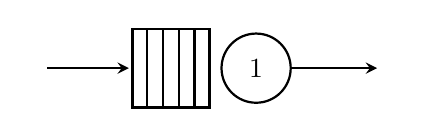
\begin{tikzpicture}[->,>=stealth,shorten >=1pt,auto,node distance=1cm,thick,main node/.style={scale=0.8,circle,draw,font=\sffamily\normalsize}]
            \node[state] (s1) []{$1$};
            \node[queue] (b1) [left of = s1]{};
            \node[] (l1) [left of = b1, xshift=-20]{};
            \node[] (x1) [right of = s1, xshift=20]{};

            \path[every node/.style={font=\sffamily\small}]
                (l1) edge (b1.west)
                (s1.east) edge (x1)
                ;
        \end{tikzpicture}

        \caption{A simple open system with a single device.}
    \end{figure}
    
    Based on the size $M_Q$ of the queue, this device could be in different states. For instance, if $M_Q = 3$, the device can be in $5$ different states:
    \begin{enumerate}[start=0]
        \item The device is idle and the queue is empty (0 jobs in the device)
        \item The device is busy and the queue is empty (1 job in the device)
        \item The device is busy and the queue contains one job (2 jobs in the device)
        \item The device is busy and the queue contains two jobs (3 jobs in the device)
        \item The device is busy and the queue contains three jobs (4 jobs in the device)
    \end{enumerate}

    In general, for a finite queue we'll always have $M_Q + 2$ states. If the queue has infinite size, we'll have an infinite number of states. After defining the population states of the device, we can discuss the idea of \textit{transitioning} from a state to another.
    
    Suppose that we know that with probability $0.5$ a new job will enter the device after a fixed time interval. Suppose that we also know that with probability $0.7$ a job will exit the device. Naively, we could think that this is enough to define a model with proper transitions froma state to another. However, these probabilities do not suffice. For instance, suppose that a job enters the device when another one is exiting it. Intuitively, the population of the device will be the same as before. Therefore, we have to be more precise: we must talk about probabilities of \textit{increasing} and \textit{decreasing} the population of the device.

    Consider now the following example. We have an open system composed by a single device with queue size $M_Q = 3$. We know that the probability of having a population increase is $0.3$, while the probability of having a population decrease is $0.4$. Is this information enough to model a correct system? The answer is yes!

    For instance, suppose that we're in state 2 (one job in the device, one in the queue). We know that with probability $0.3$ we'll transition to state 3 (one job in the device, two in the queue) and with probability $0.4$ we'll transition to state 1 (one job in the device, no jobs in the queue). However, this information allows us to infer that with probability $1-0.3-0.4 = 0.3$ we'll stay in the same state ($1-0.3 = 0.7$ and $1-0.4 = 0.6$ for states 0 and 5).

    \begin{figure}[H]
        \centering

        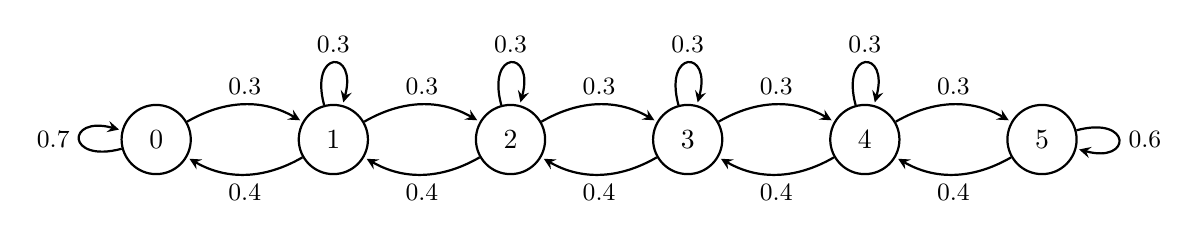
\begin{tikzpicture}[->,>=stealth,shorten >=1pt,auto,node distance=2.25cm,thick,main node/.style={scale=0.8,circle,draw,font=\sffamily\normalsize}]

            \node[state] (0) []{$0$};

            \foreach \curr [
                evaluate = \curr as \prev using {int(\curr-1)}
            ] in {1,...,5}{
                \node[state] (\curr) [right of = \prev]{$\curr$};

                \path[every node/.style={font=\sffamily\small}]
                    (\prev) edge[bend left] node{$0.3$} (\curr)
                    (\curr) edge[bend left] node{$0.4$} (\prev)
                ;
            }

            \foreach \curr in {1,...,4}{
                \path[every node/.style={font=\sffamily\small}]
                    (\curr) edge[loop above] node{$0.3$} (\curr)
                ;   
            }

            \path[every node/.style={font=\sffamily\small}]
                (0) edge[loop left] node{$0.7$} (0)
                (5) edge[loop right] node{$0.6$} (5)
            ;   

        \end{tikzpicture}

        \caption{A Markov chain describing the previous example.}
    \end{figure}
    
    This is due to the fact that the sum of outgoing probabilities of each state must be equal to 1. This property follows in a natural way from the fact that from each state we \underline{must} move to a another state (which could be itself) since the system must \curlyquotes{act} on each time interval.

    After giving the intuition behind how Markov chains work, we're ready to formally define them through \textbf{stochastic processes}, i.e. sequences $X_1, \ldots, X_n$ of random variables.

    \begin{frameddefn}{Discrete-time Markov Chain}
        We define a discrete-time Markov chain (DTMC) as an infinite stochastic process $X_1, X_2, \ldots$ such that:
        \begin{itemize}
            \item $\mathcal{I}$ is the state space
            \item $\forall n \in \N$, $X_n$ is the random variable ranging over $\mathcal{I}$ and describing the state of the system at (discrete) time step $n$.
            \item The Markovian property holds for each state, meaning that $\forall n \in \N$, $\forall j, i \in \mathcal{I}$ and $\forall i_{n-1}, \ldots, i_0 \in \mathcal{I}$ it holds that:
            \[\Pr[X_{n+1} = j \mid X_{n} = i, X_{n-1} = t_{n-1}, \ldots, X_0 = t_0] = \Pr[X_{n+1} = j \mid X_{n} = i]\]
        \end{itemize}
    \end{frameddefn}

    We observe that the Markovian property states that the probability that the conditional distribution of any future state $X_{n+1}$, given past states $X_0, X_1, \ldots , X_{n-1}$ and the present state $X_n$, is independent of past states and depends only on the present state $X_n$. This key property models the fact that from each state $i$ of the graph we can move to its adjacent states independently of how we got to state $i$ itself.

    We also observe that the Markovian property implies that the probability of transitioning from state $i$ to state $j$ is completely independent of the time step $n$. In other words, $\forall n \in \N$ it holds that:
    \[\Pr[X_{n+1} = j \mid X_n = i] = \Pr[X_n = j \mid X_{n-1} = i] = \ldots = \Pr[X_1 = j \mid X_0 = i]\]
    
    This allows us to work with the probabilities of each transition in a more concisive way by defining a \textbf{probability transition matrix} associated with each DMTC.

    \begin{frameddefn}{Probability transition matrix}
        Given a DMTC $M$ with state space $\mathcal{I}$, we define the probability transition matrix (PTM) of $M$ as the $\abs{\mathcal{I}} \times \abs{\mathcal{I}}$ matrix $P$ whose $(i,j)$-th entry $P_{i,j}$ is such that:
        \[P_{i,j} = \Pr[X_{n+1} = j \mid X_n = i]\]
    \end{frameddefn}

    \begin{figure}[H]
        \centering
        \begin{blockarray}{ccccccc}
            & \color{gray}{0} & \color{gray}{1} & \color{gray}{2} & \color{gray}{3} & \color{gray}{4} & \color{gray}{5} \\
            \begin{block}{c [*{6}{c}]}
                \color{gray}{0} & $0.7$ & $0.3$ & $0$   & $0$   & $0$   & $0$ \bigstrut[t]  \\
                \color{gray}{1} & $0.4$ & $0.3$ & $0.3$ & $0$   & $0$   & $0$   \\
                \color{gray}{2} & $0$   & $0.4$ & $0.3$ & $0.3$ & $0$   & $0$   \\
                \color{gray}{3} & $0$   & $0$   & $0.4$ & $0.3$ & $0.3$ & $0$   \\
                \color{gray}{4} & $0$   & $0$   & $0$   & $0.4$ & $0.3$ & $0.3$ \\
                \color{gray}{5} & $0$   & $0$   & $0$   & $0$   & $0.4$ & $0.6$ \\
            \end{block}
        \end{blockarray}
        \caption{The probability transition matrix of the previous example.}
    \end{figure}

    By our previous observation, we know that the probabilities of the outgoing edges of each state must sum up 1. This is equivalent to saying that the rows of each probability transition matrix must sum up to 1, i.e. $\forall i \in \mathcal{I}$ it must hold that:
    \[\sum_{j \in \mathcal{I}} P_{i,j} = 1\]

    To get familiar with how to model problems through Markov chains, we'll give an examples. Consider a facility with some machines, where each machine is either working or in the repair center. If the machine is working today, then there is a 95\% chance that it will be working tomorrow. If it is in the repair center today, then there is a 40\% chance that it will be working tomorrow. We are interested in questions like \curlyquotes{what fraction of time does my machine spend in the repair shop?}

    To model this problem, two states suffice: one for when the machine is working and one for when it is broken, respectively labeled as $W$ and $B$. From the given information, we know that $P_{W,W} = 0.95$ and $P_{B,W} = 0.4$. Since the outgoing probabilities must sum up to 1 for every state, we can infer that $P_{W,B} = 1-P_{W,W} = 1-0.95 = 0.05$ and $P_{B,B} = 1-P_{B,W} = 1-0.6 = 0.4$. 

    \begin{figure}[H]
        \centering

        \begin{tabular}{ccc}
            \begin{tabular}{c}
                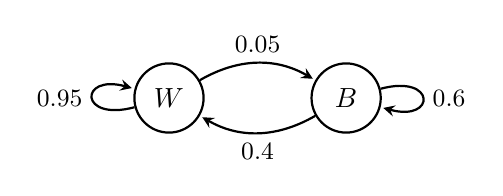
\begin{tikzpicture}[->,>=stealth,shorten >=1pt,auto,node distance=2.25cm,thick,main node/.style={scale=0.8,circle,draw,font=\sffamily\normalsize}]
                    
                    \node[state] (W) []{$W$};
                    \node[state] (B) [right of = W]{$B$};
                    
                    \path[every node/.style={font=\sffamily\small}]
                    (W) edge[loop left] node{$0.95$} (W)
                    (W) edge[bend left] node{$0.05$} (B)
                    (B) edge[loop right] node{$0.6$} (B)
                    (B) edge[bend left] node{$0.4$} (W)
                    ;
                \end{tikzpicture}
            \end{tabular}

            &\qquad\qquad&

            \begin{tabular}{c}
                \begin{blockarray}{*{3}{c}}
                & \color{gray}{$W$} & \color{gray}{$B$} \\
                    \begin{block}{c [*{2}{c}]}
                        \color{gray}{$W$} & $0.95$ & $0.05$ \bigstrut[t]  \\
                        \color{gray}{$B$} & $0.4$ & $0.6$ \\
                    \end{block}
                \end{blockarray}
            \end{tabular}
        \end{tabular}

        \caption{Model for the repair facility problem.}
    \end{figure}

    Suppose now that after the machine remains broken for 4 days, the machine is replaced with a new machine. Can we still use the same model? The answer is \underline{no}: the Markovian property explicitely affirms that the next state depends \underline{only} on the current state. In other words, Markov chains are \textbf{memoryless} by their very definition. To solve this issue, we must \curlyquotes{force} memory in the model by duplicating states. In our example, we must replace state $B$ with four states $B_1, B_2, B_3, B_4$, where, intuitively, state $B_i$ corresponds to the machine being broken for $i$ days in a row.

    \begin{figure}[H]
        \centering

        \begin{tikzpicture}[->,>=stealth,shorten >=1pt,auto,node distance=2.25cm,thick,main node/.style={scale=0.8,circle,draw,font=\sffamily\normalsize}]
            
            \node[state] (W) []{$W$};
            \foreach \curr [
                evaluate = \curr as \prev using {int(\curr-1)},
            ] in {1,...,4}{
                \node[state] (B\curr) [right of = \prev]{$B_{\curr}$};
            }

            \foreach \curr [
                evaluate = \curr as \prev using {int(\curr-1)},
                evaluate = \curr as \incurr using {int(320-(15*\prev))},
            ] in {2,...,4}{
                \path[every node/.style={font=\sffamily\small}]
                    (B\prev) edge[bend left] node{$0.6$} (\curr)
                    (B\curr) edge[out = 240, in = \incurr, near start] node{$0.4$} (W)
                ;
            }

            \path[every node/.style={font=\sffamily\small}]
                (W) edge[loop left] node{$0.95$} (W)
                (W) edge[bend left] node{$0.05$} (B1)
                (B1) edge[bend left] node{$0.4$} (W)
            ;
        \end{tikzpicture}

        \caption{Markov chain for the repair facility problem with the new rule.}
    \end{figure}

    In the previous chapter, we have discussed how in some cases it might be useful to consider the queue size as (countably) infinite. We observe that this is no issue: the definition of Markov chain doesn't restrict us to a finite number of states. In fact, we can even consider a countably infinite number of states.

    \begin{figure}[H]
        \centering

        \begin{tikzpicture}[->,>=stealth,shorten >=1pt,auto,node distance=2.25cm,thick,main node/.style={scale=0.8,circle,draw,font=\sffamily\normalsize}]

            \node[state] (0) []{$0$};

            \foreach \curr [
                evaluate = \curr as \prev using {int(\curr-1)},
                evaluate = \curr as \next using {int(\curr+1)},
            ] in {1,...,4}{
                \node[state] (\curr) [right of = \prev]{$\curr$};

                \path[every node/.style={font=\sffamily\small}]
                    (\curr) edge[bend left] node{$0.3$} (\next)
                    (\next) edge[bend left] node{$0.4$} (\curr)
                ;
            }

            \node[] (5) [right of = 4]{$\cdots$};

            \foreach \curr in {1,...,4}{
                \path[every node/.style={font=\sffamily\small}]
                    (\curr) edge[loop above] node{$0.3$} (\curr)
                ;   
            }

            \path[every node/.style={font=\sffamily\small}]
                (0) edge[loop left] node{$0.7$} (0)
                (0) edge[bend left] node{$0.3$} (1)
                (1) edge[bend left] node{$0.4$} (0)
            ;   

        \end{tikzpicture}

        \,

        \begin{blockarray}{ccccccc}
            & \color{gray}{0} & \color{gray}{1} & \color{gray}{2} & \color{gray}{3} & \color{gray}{4} & \color{gray}{$\cdots$} \\
            \begin{block}{c [*{6}{c}]}
                \color{gray}{0} & $0.7$ & $0.3$ & $0$   & $0$   & $0$   & $\cdots$ \bigstrut[t]  \\
                \color{gray}{1} & $0.4$ & $0.3$ & $0.3$ & $0$   & $0$   & $\cdots$   \\
                \color{gray}{2} & $0$   & $0.4$ & $0.3$ & $0.3$ & $0$   & $\cdots$   \\
                \color{gray}{3} & $0$   & $0$   & $0.4$ & $0.3$ & $0.3$ & $\cdots$   \\
                \color{gray}{4} & $0$   & $0$   & $0$   & $0.4$ & $0.3$ & $\cdots$ \\
                \color{gray}{$\vdots$} & $\vdots$   & $\vdots$   & $\vdots$   & $\vdots$   & $\vdots$ & $\ddots$ \\
            \end{block}
        \end{blockarray}

        \caption{A Markov chain with an infinite number of states and its PTM.}
    \end{figure}

    \section{Powers of the transition probabilities matrix}

    An absent-minded professor has two umbrellas that she uses when commuting from home to office and back. If it rains and an umbrella is available in her location, she takes it. If it is not raining, she always forgets to take an umbrella. Suppose that it rains with probability $p$ each time she commutes, independently of prior commutes. Our eventual goal is to determine the fraction of commutes during which the professor gets wet.

    First of all, we start by modeling the problem through a Markov chain. We observe that three states $0, 1, 2$ suffice: each state $i$ tracks the number of umbrellas available to the professor at the current location, regardless of what this current location is. To model the probabilities of each state, we have to carefully consider each situation:
    \begin{itemize}
        \item If our current location has no umbellas, both umbrellas must be in the other location, which will also be our next location. 
        \item If our current location has two umbellas and it rains, we'll take an umbrella with us. Hence, one umbrella will be in the next location (the one that we're going to).
        \item If our current location has two umbellas and it doesn't rain, we won't take an umbrella with us. Hence, no umbrellas will be in the next location.
        \item If our current location has one umbrella and it rains, we'll take one umbrella with us. Hence, two umbrellas will be in the next location.
        \item If our current location has one umbrella and it doesn't rain, we won't take an umbrella with us. Hence, one umbrella will be in the next location.
    \end{itemize}

    Hence, we can model the problem as follows.

    \begin{figure}[H]
        \centering

        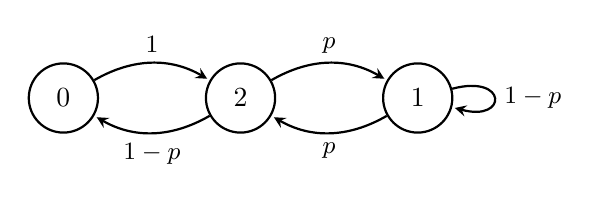
\begin{tikzpicture}[->,>=stealth,shorten >=1pt,auto,node distance=2.25cm,thick,main node/.style={scale=0.8,circle,draw,font=\sffamily\normalsize}]
            
            \node[state] (0) []{$0$};
            \node[state] (2) [right of = 0]{$2$};
            \node[state] (1) [right of = 2]{$1$};
            
            \path[every node/.style={font=\sffamily\small}]
                (0) edge[bend left] node{$1$} (2)
                (2) edge[bend left] node{$p$} (1)
                (2) edge[bend left] node{$1-p$} (0)
                (1) edge[bend left] node{$p$} (2)
                (1) edge[loop right] node{$1-p$} (1)
            ;
        \end{tikzpicture}

        \caption{Markov chain for the umbrella problem.}
        \label{umbrella_chain}
    \end{figure}


    Consider now the probability transition matrix $P$ associated with the DTMC.

    \begin{figure}[H]
        \centering

        $P = $ \begin{blockarray}{cccc}
            & \color{gray}{0} & \color{gray}{1} & \color{gray}{2} \\
            \begin{block}{c [ccc]}
                \color{gray}{0} & $0$     & $0$     & $1$      \bigstrut[t] \\
                \color{gray}{1} & $0$     & $1-p$   & $p$                  \\
                \color{gray}{2} & $1-p$   & $p$     & $0$                  \\
            \end{block}
        \end{blockarray}
        \caption{PTM for the umbrella problem.}
        \label{umbrella_ptm}
    \end{figure}

    The problem's request is to compute the probability that the professor gets wet. From our model, we know that:
    \[\Pr[\text{prof. gets wet at step $n$}] = \Pr[X_n = 0] \Pr[\text{it rains}] = \pi_0^{(n)} p\]

    where $\pi_0^{(n)} = \Pr[X_n = 0]$. To answer the request, we simply have to take the limit as $n \to +\infty$:
    \[\lim_{n \to +\infty} \Pr[\text{prof. gets wet at step $n$}] = \lim_{n \to +\infty} \pi_0^{(n)} p = \pi_0 p\]

    where $\pi_0$ is the value of $\pi_0^{(n)}$ as $n \to +\infty$. But how can be compute $\pi_0$, yet alone $\pi_0^{n}$? Through total probability, for each state $j \in \{0,1,2\}$ we get that:
    \[\begin{split}
        \pi_j^{(n)} &= \sum_{i = 0}^2 \Pr[X_n = j \mid X_{n-1} = i] \\
        & = \sum_{i = 0}^2 P_{j,i} \pi_{i}^{(n-1)}
    \end{split}\]

    Our equation is therefore structured in a recursive way. Consider now the row vector $\pi^{(n)} = \smat{\pi_0^{(n)} & \pi_1^{(n)} & \pi_2^{(n)}}$. From our previous observation, we get that:
    \[\pi^{(n)}  = \smat{\pi_0^{(n-1)} & \pi_1^{(n-1)} & \pi_2^{(n-1)}} \smat{
        0   & 0   & 1 \\
        0   & 1-p & p \\
        1-p & p   & 0}
    = \pi^{(n-1)} P\]

    By unrolling the recursive equation, we get that $\pi^{(n)} = \pi^{(0)}P^n$. To give an intuition behind what $P^n$ represents, consider the matrix $P^2$:
    \[P^2 = \smat{
        0   & 0   & 1 \\
        0   & 1-p & p \\
        1-p & p   & 0} \smat{
        0   & 0   & 1 \\
        0   & 1-p & p \\
        1-p & p   & 0} =
        \smat{
        1-p   & p         & 0 \\
        p-p^2 & 2p^2-2p+1 & p-p^2 \\
        0 & p-p^2     & p^2-p+1}\]

    Here, each entry $P^2_{i,j}$ -- short form of $(P^2)_{i,j}$ -- is given by:
    \[P^2_{i,j} = P_{i,0} P_{0,j} + P_{i,1} P_{1,j} + P_{i,2} P_{2,j}\]

    In other words, $P^2_{i,j}$ is obtained by summing the probabilities of each \textit{path} with length 2 over the Markov chain. In a similar fashion, for each $n$ we have that:
    \[P^n_{i,j} = P_{i,0} P^{n-1}_{0,j} + P_{i,1} P^{n-1}_{1,j} + P_{i,2} P^{n-1}_{2,j}\]
    
    Therefore, we can conclude that $P^n$ represents the \textbf{$n$-step probability transition matrix}, that being the matrix whose entries $P^n_{j,i}$ represent the probability of going to state $j$ from state $i$ in after $n$ (discrete) time steps, that being $P^n_{j,i} = \Pr[X_n = j \mid X_0 = i]$.

    \begin{frameddefn}{$n$-step probability transition matrix}
        Given a DMTC $M$ with state space $\mathcal{I}$, we define the $n$-step probability transition matrix of $M$ as the $n$-th power $P^n$ of its PTM $P$. In particular, for each $n > 1$ and each $i,j \in \mathcal{I}$ it holds that:
        \[P^n_{j,i} = \sum_{k \in \mathcal{I}} P^{n-1}_{j,k} P_{k,j}\]
    \end{frameddefn}

    To make things easier, we set $p = 0.4$, obtaining the following values for $P$ and $P^2$:
    \[P = \smat{
        0   & 0   & 1 \\
        0   & 0.6 & 0.4 \\
        0.6 & 0.4 & 0}
    \qquad
    P^2 = \smat{
        0.6  & 0.4   & 0 \\
        0.24 & 0.52 & 0.24 \\
        0    & 0.24 & 0.76}\]

    Let's compute some more powers (truncating values up to the third decimal):
    \[P^5 \approx \smat{
        0.057 & 0.307 & 0.635 \\
        0.184 & 0.377 & 0.438 \\
        0.381 & 0.438 & 0.180}
    \qquad
    P^{10} \approx \smat{
        0.302 & 0.412 & 0.285 \\
        0.247 & 0.391 & 0.361 \\
        0.171 & 0.361 & 0.466 \\}
    \]
    \[P^{20} \approx \smat{
        0.242 & 0.389 & 0.368 \\
        0.233 & 0.385 & 0.380 \\
        0.221 & 0.380 & 0.397}
    \qquad
    P^{30} \approx \smat{
        0.232 & 0.385 & 0.382 \\
        0.231 & 0.384 & 0.384 \\
        0.229 & 0.384 & 0.386}\]

    Therefore, we can conclude that as $n \to +\infty$ it holds that:
    \[P^{\infty} = \lim_{n \to +\infty} P^n = \smat{
        0.230 & 0.385 & 0.385 \\
        0.230 & 0.385 & 0.385 \\
        0.230 & 0.385 & 0.385}\]

    Now, let's go back to computing the vector $\pi = \smat{\pi_1 & \pi_2 & \pi_3}$ for the umbrella problem. First, we may assume that $\pi^{(0)}$ is uniform, i.e. $\pi^{(0)} = \smat{1/3 & 1/3 & 1/3}$, since each state has the same probability of being the initial one. By taking the limit of the recursive equation, we get that:
    \[\begin{split}
        \pi &= \lim_{n \to +\infty} \pi^{(0)} P^n \\
            &= \pi^{(0)} P^{\infty} \\
            &= \smat{1/3 & 1/3 & 1/3} \smat{
                0.230 & 0.385 & 0.385 \\
                0.230 & 0.385 & 0.385 \\
                0.230 & 0.385 & 0.385} \\
            &= \smat{0.23 & 0.385 & 0.385}
    \end{split}\]

    Therefore, we conclude that each $i$-th entry of each $j$-th column of the matrix $P^{\infty}$ converges to $j$-th entry of $\pi$, regardless of the initial state. We refer to the vector $\pi$ as the \textbf{limiting distribution} of the DTMC.

    \begin{frameddefn}{Limiting distribution}
        Given a DMTC $M$ with state space $\mathcal{I}$, we define the limiting distribution of $M$ as the row vector $\pi$ with $\abs{\mathcal{I}}$ entries such that:
        \begin{itemize}
            \item $\pi_j = \lim\limits_{n \to +\infty} P^n_{j,i}$ for each pair of states $i,j \in \mathcal{I}$, where $P$ is the PTM of $M$.
            \item $\sum\limits_{j \in \mathcal{I}} \pi_j = 1$
        \end{itemize}
        Each entry $\pi_j$ is referred to as the limiting probability of being in state $j$.
    \end{frameddefn}

    After computing the limiting distribution $\pi$, we can finally answer the initial question of the problem:
    \[\lim_{n \to +\infty} \Pr[\text{prof. gets wet at step $n$}] = \pi_0 p = 0.23 \cdot 0.4 = 0.092\]

    concluding that the professor gets wet on any given day is almost 10\%.

    As defined, $\pi$ is a limit. Yet it is not at all obvious that $\pi$ represents a distribution (meaning that $\sum_{j \in \mathcal{I}} \pi_j = 1$), although this turns out to be easy to see understand thanks to the previous example.

    More importantly, it is also not obvious that the limit $\pi$ even exists! For instance, consider the following Markov chain.

    \begin{figure}[H]
        \centering

        \begin{tabular}{ccc}
            \begin{tabular}{c}
                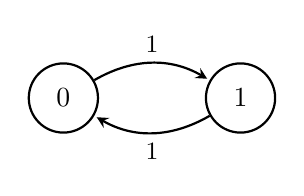
\begin{tikzpicture}[->,>=stealth,shorten >=1pt,auto,node distance=2.25cm,thick,main node/.style={scale=0.8,circle,draw,font=\sffamily\normalsize}]
                    
                    \node[state] (0) []{$0$};
                    \node[state] (1) [right of = 0]{$1$};
                    
                    \path[every node/.style={font=\sffamily\small}]
                    (0) edge[bend left] node{$1$} (1)
                    (1) edge[bend left] node{$1$} (0)
                    ;
                \end{tikzpicture}
            \end{tabular}

            &\qquad\qquad&

            \begin{tabular}{c}
                \begin{blockarray}{*{3}{c}}
                & \color{gray}{$0$} & \color{gray}{$1$} \\
                    \begin{block}{c [*{2}{c}]}
                        \color{gray}{$0$} & $0$ & $1$ \bigstrut[t]  \\
                        \color{gray}{$1$} & $1$ & $0$ \\
                    \end{block}
                \end{blockarray}
            \end{tabular}
        \end{tabular}

        \caption{A Markov chain without limiting distribution.}
        \label{limit_counterex}
    \end{figure}

    By computing $P^2, P^3$ and $P^4$, we observe that:
    \[P^2 = \smat{
        1 & 0 \\
        0 & 1}
    \qquad
    P^3 = \smat{
        0 & 1 \\
        1 & 0} = P
    \qquad
    P^4 = \smat{
        1 & 0 \\
        0 & 1} = P^2\]

    This implies that for each $k \in \N$ it holds that $P^{2k} = P^2$ and $P^{2k+1} = P^1$ and therefore that the matrix $P^{\infty} = \lim\limits_{n \to +\infty} P^n$ doesn't converge! In next sections, we'll see ways to determine if such limit exists. 
    
    \section{Stationary distribution}

    In the previous section we found out how the limiting distribution $\pi$ can be computed (when it exists) by solving the equation $\pi = \pi_0 P^{\infty}$, which is equivalent to setting $\pi_j = P^{\infty}_{j,i}$ for each $j \in \mathcal{I}$.
    
    However, computing $P^{\infty}$ is clearly a tedious task, making this process impracticable. To fix this issue, we require a faster way to compute $\pi$. Let's go back to the original recursive equation of $\pi$. We saw how for each $n$ it holds that:
    \[\pi^{(n)} = \pi^{(n-1)} P\]

    By taking the limit as $n \to +\infty$, we get that:
    \[\pi = \lim_{n \to +\infty} \pi^{(n)}= \lim_{n \to +\infty} \pi^{(n-1)} P = \pi P\]

    In other words, the PTM doesn't change the values of the limit distribution. Distributions with such property as said to be \textbf{stationary distributions} for the DTMC.

    \begin{frameddefn}{Stationary distribution}
        Given a DMTC $M$ with state space $\mathcal{I}$, a vector $v$ of $\abs{\mathcal{I}}$ entries is said to be a stationary distribution of $M$ if:
        \begin{itemize}
            \item $v = vP$, where $P$ is the PTM of $M$
            \item $\sum\limits_{j \in \mathcal{I}} v_j = 1$
        \end{itemize}
    \end{frameddefn}

    We have already concluded that the limiting distribution (when it exists) is a stationary distribution. However, a stronger result can be proven: every stationary distribution must be equal to the limiting distribution!

    \begin{framedthm}{}
        Given a DMTC $M$ (with finite or countably infinite states), if $M$ admits a limiting distribution $\pi$ then it is the unique stationary distribution.
    \end{framedthm}

    \begin{proof}
        We prove the theorem only for DMTCs with a finite number of states. We already know that (when it exists) $\pi$ is a stationary distribution, hence it suffices to prove that it is the unique stationary distribution. Let $v$ be a stationary distribution of $M$ and suppose that the limiting distribution $\pi$ exists.. Since $v$ is stationary, for each $k \in \mathcal{I}$ we have that:
        \[v_k = \Pr[X_n = k] = \ldots = \Pr[X_0 = k]\]

        Moreover, since $v_k$ contains constant values, we have that $v = \lim\limits_{n \to +\infty} v$.
        
        Now, fix any $j \in \mathcal{I}$. We observe that:
        \[\begin{split}
            v_j &= \Pr[X_n = j] \\
            &= \sum_{i \in \mathcal{I}} \Pr[X_n = j \mid X_{0} = i] \Pr[X_0 = i] \\
            &= \sum_{i \in \mathcal{I}} P^n_{j,i} v_i
        \end{split}\]

        Therefore, by taking the limit as $n \to +\infty$ we have that:
        \[v_j = \lim_{n \to +\infty} v_j = \lim_{n \to +\infty} \sum_{i \in \mathcal{I}} P^n_{j,i} v_i = \sum_{i \in \mathcal{I}} \lim_{n \to +\infty}  P^n_{j,i} v_i = \sum_{i \in \mathcal{I}} \pi_j v_i = \pi_j \sum_{i \in \mathcal{I}} v_i = \pi_j\]

        concluding that $v = \pi$.

        \textit{Note}: we observe that with a infinite number of states we cannot simply take a limit from the outside of an infinite sum to its inside since the sum might not converge. Thus, a proof for a countably infinite number of states requires to be more precise.
    \end{proof}

    The above theorem is a fundamental result in \textit{Markov theory}, allowing us to compute limiting distributions (assuming it exists) simply by solving the following system, called \textbf{stationary equations}:
    \[\soe{ll}{
        \pi = \pi P \\
        \sum_{j \in \mathcal{I}} \pi_j = 1
    }\]

    For instance consider again the umbrella problem shown in the below picture, with a generic value $p$ and its associated PTM $P$ (\Cref{umbrella_ptm}).
    
    \begin{figure}[H]
        \centering

        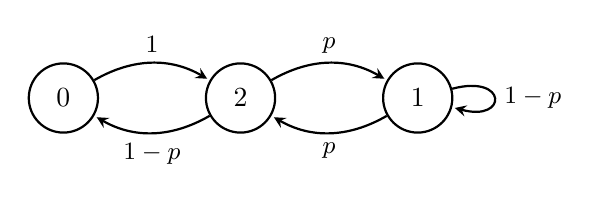
\begin{tikzpicture}[->,>=stealth,shorten >=1pt,auto,node distance=2.25cm,thick,main node/.style={scale=0.8,circle,draw,font=\sffamily\normalsize}]
            
            \node[state] (0) []{$0$};
            \node[state] (2) [right of = 0]{$2$};
            \node[state] (1) [right of = 2]{$1$};
            
            \path[every node/.style={font=\sffamily\small}]
                (0) edge[bend left] node{$1$} (2)
                (2) edge[bend left] node{$p$} (1)
                (2) edge[bend left] node{$1-p$} (0)
                (1) edge[bend left] node{$p$} (2)
                (1) edge[loop right] node{$1-p$} (1)
            ;
        \end{tikzpicture}
    \end{figure}
    
    To compute the limiting distribution, all we have to do is to solve the following system of linear equations:
    \[\soe{rl}{
        \pi_0 &= (1-p) \pi_2 \\
        \pi_1 &= (1-p) \pi_1 + p \pi_2 \\
        \pi_2 &= \pi_0 + p \pi_1 \\
        \pi_0 + \pi_1 + \pi_2 &= 1
    }\]

    which yields the following solutions:
    \[\pi_0 = \frac{1-p}{3-p} \qquad \pi_1 = \frac{1}{3-p} \qquad \pi_2 = \frac{1}{{3-p}}\]

    By setting $p = 0.4$, we get the same solution to the umbrella problem, i.e. $\pi_0 p = \frac{24}{260} \approx 0.092$, further proving the truthfulness of the theorem.

    Clearly, this method can only be used \underline{only} if we're sure that the limiting distribution exists since otherwise it is not guaranteed that every stationary distribution is the limiting one.
    
    For instance, consider again the counterexample shown in \Cref{limit_counterex}.
    
    \begin{figure}[H]
        \centering

        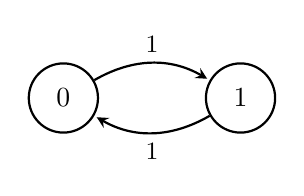
\begin{tikzpicture}[->,>=stealth,shorten >=1pt,auto,node distance=2.25cm,thick,main node/.style={scale=0.8,circle,draw,font=\sffamily\normalsize}]
            
            \node[state] (0) []{$0$};
            \node[state] (1) [right of = 0]{$1$};
            
            \path[every node/.style={font=\sffamily\small}]
            (0) edge[bend left] node{$1$} (1)
            (1) edge[bend left] node{$1$} (0)
            ;
        \end{tikzpicture}
    \end{figure}

    We've already proven that the limiting distribution for this DMTC doesn't exist. However, we can still find a stationary distribution by solving the associated system.
    \[\soe{rl}{
        \pi_0 &= \pi_1 \\
        \pi_1 &= \pi_0 \\
        \pi_0 + \pi_1 &= 1
    }\]

    which yields the solutions $\pi_0 = \pi_1 = \frac{1}{2}$. Therefore, a stationary distribution may exist even when the limiting distribution doesn't exist.

    \newpage

    \section{The barrier technique}

    Consider again the umbrella problem and its stationary equations.

    \begin{figure}[H]
        \centering

        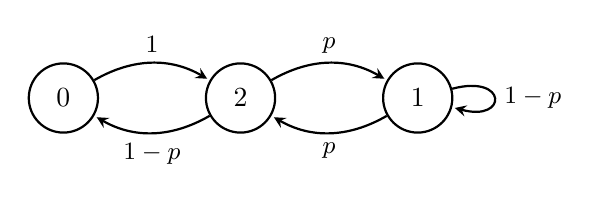
\begin{tikzpicture}[->,>=stealth,shorten >=1pt,auto,node distance=2.25cm,thick,main node/.style={scale=0.8,circle,draw,font=\sffamily\normalsize}]
            
            \node[state] (0) []{$0$};
            \node[state] (2) [right of = 0]{$2$};
            \node[state] (1) [right of = 2]{$1$};
            
            \path[every node/.style={font=\sffamily\small}]
                (0) edge[bend left] node{$1$} (2)
                (2) edge[bend left] node{$p$} (1)
                (2) edge[bend left] node{$1-p$} (0)
                (1) edge[bend left] node{$p$} (2)
                (1) edge[loop right] node{$1-p$} (1)
            ;
        \end{tikzpicture}
    \end{figure}

    \[\soe{rl}{
        \pi_0 &= (1-p) \pi_2 \\
        \pi_1 &= (1-p) \pi_1 + p \pi_2 \\
        \pi_2 &= \pi_0 + p \pi_1 \\
        \pi_0 + \pi_1 + \pi_2 &= 1
    }\]

    We observe that the second stationary equation reveals a secret fact:
    \[\pi_1 = (1-p) \pi_1 + p \pi_2 \implies p \pi_1 = p \pi_2\]

    This is no coincidence! If we consider the ingoing and outgoing probabilities of each state as \curlyquotes{flows}, it's easy to see that these two quantities must be equal. Therefore, the outgoing flow of state 2, that being $\pi_2 p$ must be equal to its ingoing flow, that being $\pi_1 p$, concluding that $p \pi_2 = p \pi_1$. This property is referred to as the \textbf{conservation of flows} between two states. Visually, it appears as if we placed a \curlyquotes{barrier} between the two transitions $(2,1)$ and $(1,2)$, hence the name \textit{barrier technique}.

    \begin{figure}[H]
        \centering

        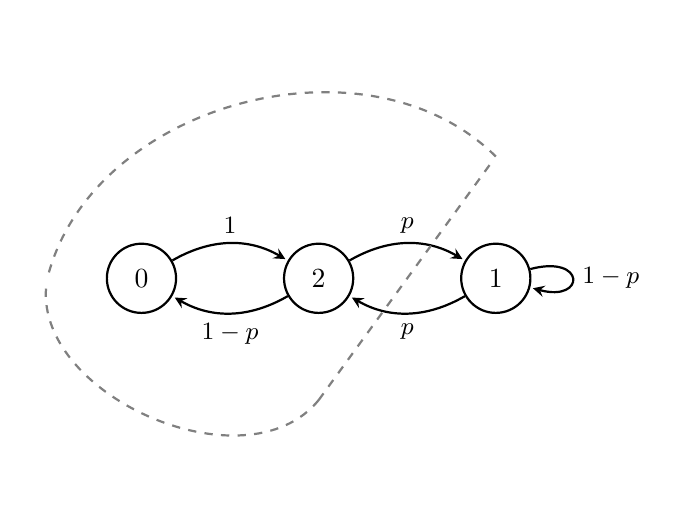
\begin{tikzpicture}[->,>=stealth,shorten >=1pt,auto,node distance=2.25cm,thick,main node/.style={scale=0.8,circle,draw,font=\sffamily\normalsize}]
            
            \node[state] (0) []{$0$};
            \node[state] (2) [right of = 0]{$2$};
            \node[state] (1) [right of = 2]{$1$};

            \node[] (x) [below of = 2, yshift=20]{};
            \node[] (y) [above of = 1, yshift=-20]{};
            \node[] (z) [left of = 0, xshift=30]{};
            
            \path[every node/.style={font=\sffamily\small}]
                (0) edge[bend left] node{$1$} (2)
                (2) edge[bend left] node{$p$} (1)
                (2) edge[bend left] node{$1-p$} (0)
                (1) edge[bend left] node{$p$} (2)
                (1) edge[loop right] node{$1-p$} (1)
            ;


            \path[-, every node/.style={font=\sffamily\small}]
                (x.center) edge[dashed, color = gray] (y.center)
                (x.center) edge[dashed, color = gray, bend left = 75] (z.center)
                (y.center) edge[dashed, color = gray, bend right = 60] (z.center)
            ;
        \end{tikzpicture}

        \caption{Visual representation of the barrier technique.}
    \end{figure}

    The barrier technique can be used to solve stability equations in a faster way by allowing us to consider simpler equations instead of the ones given by $\pi = \pi P$. For instance, consider again the Markov chain of the repair facility problem shown below.

    \begin{figure}[H]
        \centering

        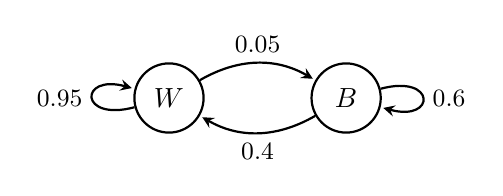
\begin{tikzpicture}[->,>=stealth,shorten >=1pt,auto,node distance=2.25cm,thick,main node/.style={scale=0.8,circle,draw,font=\sffamily\normalsize}]
            
            \node[state] (W) []{$W$};
            \node[state] (B) [right of = W]{$B$};
            
            \path[every node/.style={font=\sffamily\small}]
            (W) edge[loop left] node{$0.95$} (W)
            (W) edge[bend left] node{$0.05$} (B)
            (B) edge[loop right] node{$0.6$} (B)
            (B) edge[bend left] node{$0.4$} (W)
            ;
        \end{tikzpicture}
    \end{figure}

    To find the limiting probability in the usual way, we solve the following system.
    \[\soe{ll}{
        \pi_0 &= 0.95 \cdot \pi_0 + 0.4 \cdot \pi_1 \\
        \pi_1 &= 0.05 \cdot \pi_0 + 0.6 \cdot \pi_1 \\
        \pi_0 + \pi_1 &= 1
    }\]

    By solving the system, we get that $\pi_0 = 0.875$ and $\pi_1 = 0.125$. Now, we'll find these same results by applying the barrier technique. Since the two transitions $(W,B)$ and $(B,W)$ exists, we know that the ingoing flow must be equal to the outgoing flow, allowing us to apply the barrier technique.

    \begin{figure}[H]
        \centering

        \begin{tikzpicture}[->,>=stealth,shorten >=1pt,auto,node distance=2.25cm,thick,main node/.style={scale=0.8,circle,draw,font=\sffamily\normalsize}]
            
            \node[state] (W) []{$W$};
            \node[state] (B) [right of = W]{$B$};
            \node[] (x) [below of = W, yshift=20]{};
            \node[] (y) [above of = B, yshift=-20]{};
            \node[] (z) [left of = 0]{};
            
            \path[every node/.style={font=\sffamily\small}]
            (W) edge[loop left] node{$0.95$} (W)
            (W) edge[bend left] node{$0.05$} (B)
            (B) edge[loop right] node{$0.6$} (B)
            (B) edge[bend left] node{$0.4$} (W)
            ;

            \path[-, every node/.style={font=\sffamily\small}]
                (x.center) edge[dashed, color = gray] (y.center)
                (x.center) edge[dashed, color = gray, bend left = 60] (z.center)
                (y.center) edge[dashed, color = gray, bend right = 60] (z.center)
            ;
        \end{tikzpicture}
        \caption{Application of the barrier technique on the repair facility problem.}
    \end{figure}

    Therefore, we get that $0.05 \cdot \pi_W = 0.4 \cdot \pi_B$ must hold. Moreover, we know that $\pi$ must be a distribution, i.e. the sum of all of its entries must be equal to 1. This gives us a new smaller system of equations from which we can immediately conclude that $\pi_0 = 0.875$ and $\pi_1 = 0.125$:
    \[\soe{ll}{
        0.05 \cdot \pi_W &= 0.4 \cdot \pi_B  \\
        \pi_0 + \pi_1 &= 1
    }\]
    
    For bigger chains, the barrier technique allows us to reduce the number of computations by an extreme amount. For instance, consider the following Markov chain.


    \begin{figure}[H]
        \centering

        \resizebox{1\textwidth}{!}{
            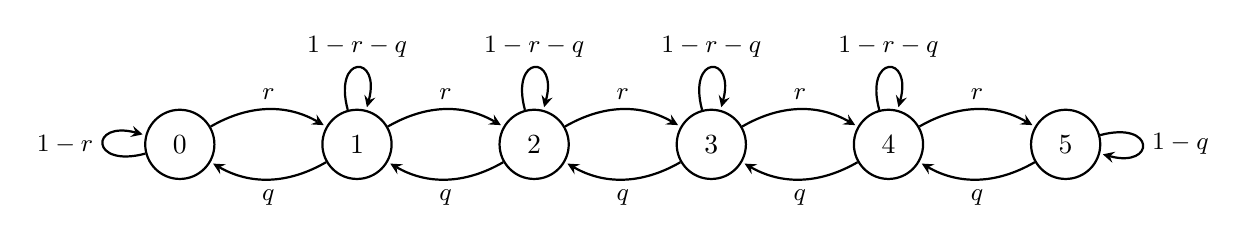
\begin{tikzpicture}[->,>=stealth,shorten >=1pt,auto,node distance=2.25cm,thick,main node/.style={scale=0.8,circle,draw,font=\sffamily\normalsize}]

                \node[state] (0) []{$0$};

                \foreach \curr [
                    evaluate = \curr as \prev using {int(\curr-1)}
                ] in {1,...,5}{
                    \node[state] (\curr) [right of = \prev]{$\curr$};

                    \path[every node/.style={font=\sffamily\small}]
                        (\prev) edge[bend left] node{$r$} (\curr)
                        (\curr) edge[bend left] node{$q$} (\prev)
                    ;

                }

                \foreach \curr in {1,...,4}{
                    \path[every node/.style={font=\sffamily\small}]
                        (\curr) edge[loop above] node{$1-r-q$} (\curr)
                    ;   
                }

                \path[every node/.style={font=\sffamily\small}]
                    (0) edge[loop left] node{$1-r$} (0)
                    (5) edge[loop right] node{$1-q$} (5)
                ;   

            \end{tikzpicture}
        }
    \end{figure}

    By applying the barrier technique on each pair of states $(i-1,i)$, with $i \in [5]$, we obtain:
    \[r \pi_{i-1} = \pi_{i} q \implies \pi_{i} = \frac{r}{q} \pi_{i-1} \qquad \forall i \in [5]\]
    
    \begin{figure}[H]
        \centering

        \resizebox{1\textwidth}{!}{
            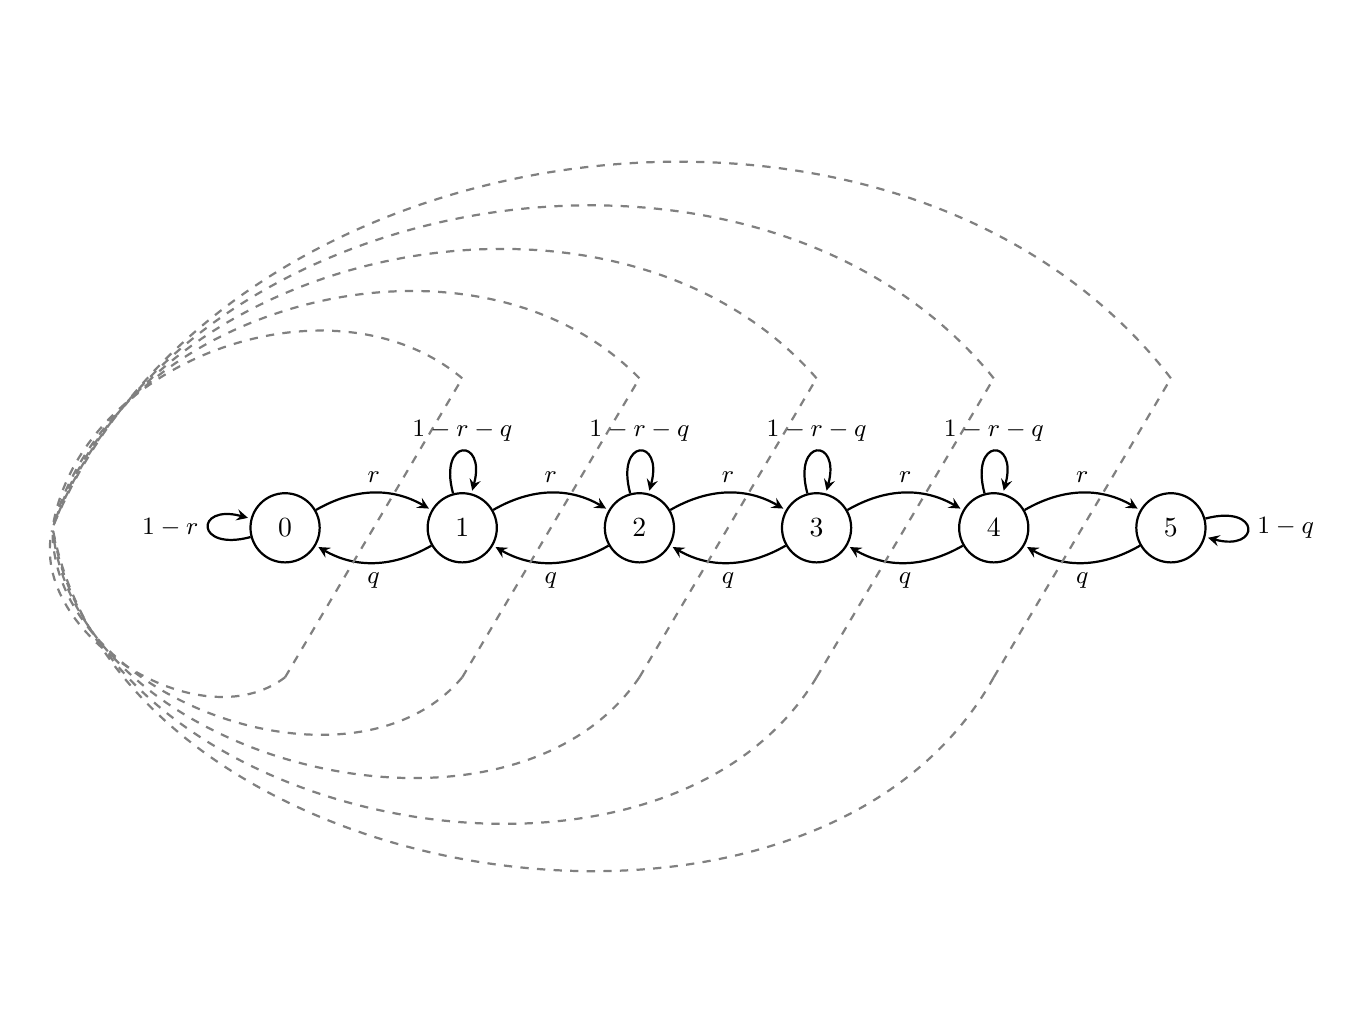
\begin{tikzpicture}[->,>=stealth,shorten >=1pt,auto,node distance=2.25cm,thick,main node/.style={scale=0.8,circle,draw,font=\sffamily\normalsize}]

                \node[state] (0) []{$0$};
                \node[] (z) [left of = 0, xshift = -20]{};

                \foreach \curr [
                    evaluate = \curr as \prev using {int(\curr-1)}
                ] in {1,...,5}{
                    \node[state] (\curr) [right of = \prev]{$\curr$};
                    \node[] (x\prev) [below of = \prev, yshift=10]{};
                    \node[] (y\curr) [above of = \curr, yshift=-10]{};

                    \path[every node/.style={font=\sffamily\small}]
                        (\prev) edge[bend left] node{$r$} (\curr)
                        (\curr) edge[bend left] node{$q$} (\prev)
                    ;

                    \path[-, every node/.style={font=\sffamily\small}]
                        (x\prev.center) edge[dashed, color = gray] (y\curr.center)
                        (x\prev.center) edge[dashed, color = gray, bend left = 70] (z.center)
                        (y\curr.center) edge[dashed, color = gray, bend right = 60] (z.center)
                    ;
                }

                \foreach \curr in {1,...,4}{
                    \path[every node/.style={font=\sffamily\small}]
                        (\curr) edge[loop above] node{$1-r-q$} (\curr)
                    ;   
                }

                \path[every node/.style={font=\sffamily\small}]
                    (0) edge[loop left] node{$1-r$} (0)
                    (5) edge[loop right] node{$1-q$} (5)
                ;   

            \end{tikzpicture}
        }

        \caption{Graphical representation of multiple applications of the barrier technique. Each barrier is independent from the others, meaning that the inside and outside of a barrier should be considered without the other barriers.}
    \end{figure}

    By adding the condition $\sum\limits_{i = 0}^5 \pi_i = 1$, we get the following system of equations:
    \[\soe{rlcl}{
        \pi_{i} &= \dfrac{r}{q} \pi_{i-1} & \qquad & \forall i \in [5] \\
        \sum\limits_{i = 0}^5 \pi_i &= 1
    }\]

    Now, let $\rho = \dfrac{r}{q}$. By unrolling the recursive equation up to $\pi_0$, we get that:
    \[\soe{rlcl}{
        \pi_{i} &= \rho^i \pi_{0} & \qquad & \forall i \in [5] \\
        \sum\limits_{i = 0}^5 \pi_i &= 1
    }\]

    By substituting the unrolled equation into the sum, we get that:
    \[1 = \sum\limits_{i = 0}^5 \pi_i  = \sum\limits_{i = 0}^5 \rho^i \pi_0  = \pi_0 \sum\limits_{i = 0}^5 \rho^i  = \pi_0 \cdot \frac{1-\rho^6}{1-\rho}\]

    where the last step is due to the finite geometric sum:
    \[\sum_{i = 0}^n x^i = \frac{1-x^{n+1}}{1-x}\]

    Therefore, we get that:
    \[\soe{rlcl}{
        \pi_{i} &= \rho^i \pi_{0} & \qquad & \forall i \in [5] \\
        \rho_0 &= \dfrac{1-\rho}{1-\rho^6}
    }\]

    and thus that:
    \[\pi_{i} = \dfrac{\rho^i(1-\rho)}{1-\rho^6} \qquad \forall i \in \{0, \ldots, 5\}\]


    \section{Existence of limiting distributions}

    In the previous chapter we introduced performance analysis through Markov chains, observing that it may not always be true that a limiting distribution exists. In this section, we'll discuss how \textbf{ergodicity} ensures the existence of such limit. We already introduced the concept of ergodicity in the first chapter, stating that a system is ergodic when it is irreducible, positive recurrent and aperiodic. Now, we'll give the corresponding definitions for this three properties in the case of Markov chains.

    We start with the simplest one: \textbf{aperiodicity}. We said that \curlyquotes{the system is aperiodic if it never returns in a specific state after a precise amount of time}. To understand how this applies to Markov chains, consider the following example.

    \begin{figure}[H]
        \centering
        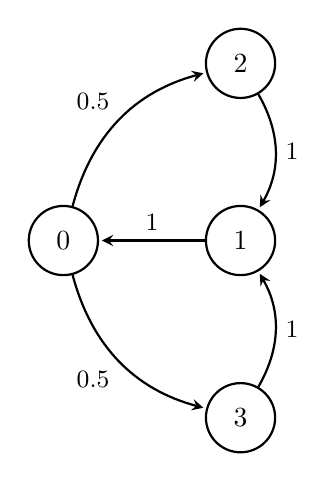
\begin{tikzpicture}[->,>=stealth,shorten >=1pt,auto,node distance=2.25cm,thick,main node/.style={scale=0.8, circle,draw,font=\sffamily\normalsize}]

            \node[state] (0) []{$0$};
            \node[state] (1) [right of = 0]{$1$};
            \node[state] (2) [above of = 1]{$2$};
            \node[state] (3) [below of = 1]{$3$};

            \path[every node/.style={font=\sffamily\small}]
                (0) edge[bend left] node{$0.5$} (2)
                (0) edge[bend right, swap] node{$0.5$} (3)
                (2) edge[bend left] node{$1$} (1)
                (3) edge[bend right, swap] node{$1$} (1)
                (1) edge[swap] node{$1$} (0)
            ;
        \end{tikzpicture}

        \caption{A periodic Markov chain.}
    \end{figure}

    It's easy to see that this chain is periodic: if we start from state $0$, it will return to this state every 3 time steps, independently of the transitions that it took. Now, observe what happens to the $3$-step PTM:
    \[P = \smat{
        0 & 0 & 0.5 & 0.5   \\
        1 & 0 & 0   & 0     \\
        0 & 1 & 0   & 0     \\
        0 & 1 & 0   & 0     
    } \implies P^3 = \smat{
        1 & 0 & 0    & 0     \\
        0 & 1 & 0   & 0     \\
        0 & 0 & 0.5 & 0.5   \\
        0 & 0 & 0.5   & 0.5   
    }\]

    We notice that the main diagonal of the matrix is filled with non-zero entries, meaning that every state has a non-zero probability of going back to itself in 3 steps. In particular, states 0 and 1 will surely go back to themselves every 3 steps. This allows us to define the idea of \textit{state period}.

    \begin{frameddefn}{State period}
        Given a DMTC $M$ with state space $\mathcal{I}$ and PTM $P$, we define the period of state $i \in \mathcal{I}$ as the GCD of the set $\{n \in \N \mid P_{i,i}^n > 0\}$. A state is said to be aperiodic if its period is 1. The chain $M$ is said to be aperiodic if every state is aperiodic.
    \end{frameddefn}

    After defining periodicity, we make some observations on this definition. First of all, we have to clarify things: we said that a state is aperiodic if it has period 1, but shouldn't value set to zero in order to be aperiodic? Let's take a step back to the initial definition of aperiodicity: \curlyquotes{the system is aperiodic if it never returns in a specific state after a precise amount of time}. If the period of a state $i$ is 1, we have two possibilities:
    \begin{itemize}
        \item The GCD of the set $\{n \in \N \mid P_{i,i}^n > 0\}$ is equal to 1 because each value of the set is bigger than 1 and pair-wise coprime. This coprimality guarantees that not every value of the set is a multiple of a specific number, breaking periodicity. 
        \item The GCD of the set $\{n \in \N \mid P_{i,i}^n > 0\}$ is equal to 1 because 1 is inside the set. This can happen only if state $i$ has a loop in the chain with non-zero probability. This guarantees that it has a probability of returning to iself \underline{every single time step}, thus everything that may happen in time step $i$ is may also happen in time step $i+1$, breaking periodicity.
    \end{itemize}
    
    After clarifying the definition of aperiodicity, let's consider some practical examples. Consider again the Markov chain of the umbrella problem, shown below.

    \begin{figure}[H]
        \centering

        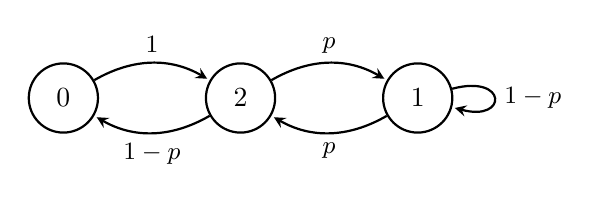
\begin{tikzpicture}[->,>=stealth,shorten >=1pt,auto,node distance=2.25cm,thick,main node/.style={scale=0.8,circle,draw,font=\sffamily\normalsize}]
            
            \node[state] (0) []{$0$};
            \node[state] (2) [right of = 0]{$2$};
            \node[state] (1) [right of = 2]{$1$};
            
            \path[every node/.style={font=\sffamily\small}]
                (0) edge[bend left] node{$1$} (2)
                (2) edge[bend left] node{$p$} (1)
                (2) edge[bend left] node{$1-p$} (0)
                (1) edge[bend left] node{$p$} (2)
                (1) edge[loop right] node{$1-p$} (1)
            ;
        \end{tikzpicture}
    \end{figure}

    Let $p = 0.4$. Then, the state $1$ has a loop with non-zero probability, concluding immediately that its period is 1. To compute the period of states 0 and 2, we take some powers of $P$:
    \[P = \smat{
        0   & 0   & 1 \\
        0   & 0.6 & 0.4 \\
        0.6 & 0.4 & 0
    } \qquad
    P^2 \approx \smat{
        0.6  & 0.4   & 0 \\
        0.24 & 0.52 & 0.24 \\
        0    & 0.24 & 0.76
    } \qquad 
    P^3 \approx \smat{
        0 & 0.24 & 0.76 \\
        0.14 & 0.41 & 0.45 \\
        0.46 & 0.45 & 0.10 \\
    }\]
    \[P_4 \approx \smat{
        0.46 & 0.45 & 0.10 \\
        0.27 & 0.42 & 0.31 \\
        0.06 & 0.31 & 0.63 \\
    }\qquad 
    P_5 = \smat{
        0.06 & 0.31 & 0.63 \\
        0.19 & 0.38 & 0.44 \\
        0.38 & 0.44 & 0.18
    } \qquad
    P_6 \approx \smat{
        0.38 & 0.44 & 0.18 \\
        0.26 & 0.40 & 0.33 \\
        0.11 & 0.33 & 0.56
    }\]

    From these few powers, it already seems that for every $n \in \N$ and every $i \in \{0,1,2\}$ it holds that $P_{i,i}^n > 0$, concluding that the period of every state is 1 and thus concluding that the chain is aperiodic. This is no coincidence: the small loop of state 1 is sufficient to make the whole chain aperiodic. First, we give some definition.
    
    \begin{frameddefn}{Accessibility and communication}
        Consider a DMTC $M$ with state space $\mathcal{I}$. Given a pair $i,j \in \mathcal{I}$, we say that state $j$ is accessible from state $i$ if $P_{i,j}^n > 0$ for some $n \in \N$. Similarly, we say that states $i$ and $j$ communicate if $i$ is accessible from $j$ and vice versa.
    \end{frameddefn}

    The above definitions and the previous observation make the following concludion pretty obvious: if a state is aperiodic and another state communicates with it, the latter state can use the aperiodicity of the former state to break its own periodicity.

    \begin{framedprop}{}
        Consider a DMTC $M$ with state space $\mathcal{I}$. If state $i \in \mathcal{I}$ is aperiodic, every state $j \in \mathcal{I}$ that communicates with $i$ is also aperiodic.
    \end{framedprop}

    \begin{proof}
        Omitted.
    \end{proof}

    After understanding aperiodicity, let's move to \textbf{irreducibility}. We said that \curlyquotes{a system is irreducible if from every state the system can reach every other state and back}. After defining the concept of communication, the definition of irreducible Markov chain is straight forward.

    \begin{frameddefn}{Irreducible Markov chain}
        A Markov chain is said to be irreducible if each pair of states communicate with each other. 
    \end{frameddefn}

    This leaves us with defining \textbf{positive recurrence}. For now, we defer the discussion about positive recurrence. In fact, for finite-state DTMC, irreducibility and aperiodicity is all we need to guarantee that a limiting distribution exists!
    
    \begin{framedthm}{Existence of lim. distibution (finite case)}
        Consider a DMTC $M$ with finite state space $\mathcal{I}$ and PTM $P$. If $M$ is irreducible and aperiodic then $\lim\limits_{n \to +\infty} P^n$ exists and corresponds to a matrix $L$ whose rows are all equal to the limiting distribution of $M$. 
    \end{framedthm}
    
    \begin{proof}
        Fix $j \in [\abs{\mathcal{I}}]$. Let $e_j$ be the column vector whose entries are all set to 0 except for the $j$-th entry, which is set to 1. We observe that for each $n \in \N$ the product $P^ne_j$ corresponds to the $j$-th column of $P^n$.
        
        Fix $n \in \N$. Let $M_n$ and $m_n$ be, respectively, the maximum and minimum value of any component of $P^n e_j$. Similarly, let $s$ be the smallest element of the whole matrix $P$.
        
        \textit{Note}: we observe that these values are guaranteed to exist only on a finite state Markov chain, making this proof invalid for infinite state ones.

        \textbf{Claim}: $M_n - m_n \leq (1-2s)(M_{n-1} - m_{n-1})$

        \begin{proof}[Proof of the claim.]
            Let $y = P^{n-1}e_j$. First, we observe that the largest possible value is obtained if all but one of the elements of $y$ are $M_{n-1}$, with the remaining one being $m_{n-1}$, where $m_{n-1}$ is weighted by the smallest value $s$. This concludes that: 
            \[M_n \leq (1-s)M_{n-1} + s m_{n-1}\]

            With a symmetrical argument, we can conclude that:
            \[m_n \geq (1-s)m_{n-1} + s M_{n-1}\]

            Summing the two inequalities, we get that:
            \[M_n - \leq (1-s)M_{n-1} + s m_{n-1} - (1-s)m_{n-1} - s M_{n-1} = (1-2s)(M_{n-1} - m_{n-1})\]
        \end{proof}

        Due to irreducibility and aperiodicity of $P$, there must be a value $n_0 \in \N$ such that $P^{n_0}$ has no null-entries. Let $P' = P^{n_0}$. We observe that the same argument used for the claim also holds for $P'$, implying that $M'_n - m'_n \leq (1-2s')(M'_{n-1} - m'_{n-1})$.

        By unrolling the recursive inequality, we get that:
        \[M'_n - m'_n \leq (1-2s')^{n-1}(M'_1 - m'_1)\]
        Now, we observe that $s' \leq 0.5$ must hold since each row of $P$ must sum up to 1. Therefore, we conclude that:
        \[0 \leq \lim_{n \to +\infty} M'_n - m'_n \leq \lim_{n \to +\infty} (1-2s')^{n-1}(M'_1 - m'_1) = 0\]

        Thus, each column $(P')^ne_j$ will eventually reach a point where all entries are equal to each other, concluding that $\lim\limits_{n \to +\infty} (P')^n$ converges to a matrix $L$ whose rows are all equal to each other, meaning that each row will be equal to the of limiting distribution of $P$.
    \end{proof}
    
    The above theorem implicitely states that positive recurrence is not needed for finite state chains. However, we're actually missing a piece of the puzzle: every irreducible finite state chain is already positive recurrent! In other words, we're actually already implicitely using positive recurrence in the theorem! To convince ourselves, recall that we said that \curlyquotes{a system is positive recurrent if starting from a state, the probability to return in that same state over infinite time is 1}. Then, for a finite state chain, irreducibility already implies that starting from a state we will eventually come back to it in a finite amount of time!

    Then why do when do we also need positive recurrence? The answer is simple: for infinite chains! To formally define positive recurrence, we first have to define a more neutral concept, i.e. \textit{recurrence}.

    \begin{frameddefn}{Recurrency and transiency}
        Consider a DMTC $M$ with state space $\mathcal{I}$. Given a state $i \in \mathcal{I}$, let $f_i$ be the probability of, eventually, returning to $i$ starting from $i$, i.e.:
        \[f_i = \Pr\sbk{\bigcup_{n = 1}^{+\infty} X_n = i \mid X_0 = i}\]
        
        We say that state $i$ is recurrent if $f_i = 1$, otherwise we say that it is transient. We say that a Markov chain is recurrent if every state is recurrent. We say that a Markov chain is transient if every state is transient.
    \end{frameddefn}

    \begin{framedprop}{}
        With probability 1, the number of visits to a recurrent state is
        infinite. With probability 1, the number of visits to a transient state is finite.
    \end{framedprop}

    \begin{proof}
        If a state $j$ is recurrent, then starting in state $j$, with probability 1 we will visit
        $j$ again. Thus, repeating this argument, we see that with probability 1 state $j$ will be
        visited an infinite number of times. In contrast, if state $j$ is transient, then every time
        we visit state $j$, there is some probability $(1 - f_j)$ that we will never again visit $j$.
        Thus, with probability 1 state $j$ will be visited a finite number of times.
    \end{proof}

    \begin{framedprop}{}
        Consider a DMTC $M$ with state space $\mathcal{I}$. If state $i \in \mathcal{I}$ is recurrent, every state $j \in \mathcal{I}$ that communicates with $i$ is also recurrent. Similarly, If state $i \in \mathcal{I}$ is transient, every state $j \in \mathcal{I}$ that communicates with $i$ is also transient.
    \end{framedprop}

    \begin{proof}
        Omitted.
    \end{proof}

    \begin{frameddefn}{Positive recurrence and null recurrence}
        Consider a DMTC $M$ with state space $\mathcal{I}$. Given a recurrent state $i \in \mathcal{I}$, let $\mu_i$ be the expected time taken to return to state $i$ when starting from $i$, i.e.:
        \[\mu_i = \sum_{n = 1}^{+\infty} n \Pr[X_n = i \mid X_0 = i]\]
        
        We say that state $i$ is positive recurrent if $\mu_i < +\infty$, otherwise we say that it is null recurrent.
    \end{frameddefn}

    The above proposition implies that in an irreducible Markov chain states are either all recurrent or transient. Without diving into mathematical details, we give a general form of the previous theorem that holds for every ergodic Markov chain.

    \begin{framedthm}{Ergodic theorem for Markov chains}
        In every ergodic Markov chain the limiting distribution exists.
    \end{framedthm}

    \begin{proof}
        Omitted.
    \end{proof}

    \newpage

    \section{Solved exercises}

    \begin{framedprob}{}
        Consider an open system formed by a single server with an unbounded queue. Suppose that, at every time step, with probabiliy $p_a$ a new job arrives to the server, while old jobs depart with probability $p_d$. Note that during a time step, we might have both an arrival and a transmission, or neither.
        
        Assuming the limiting probability exists, find the values of $\Exp[N], \Exp[N^{\text{server}}]$ and $\Exp[N^{\text{queue}}]$ without using the barrier technique.
    \end{framedprob}

    \textit{Solution:}

    Using the given data, we can compute the probabilitites $r$ and $s$ of having a population increase or decrease. A population increase happens when a new job arrives and no job departs. Similarly, a population decrease happens when a no job arrives and a job departs. Thus, we get that $r = p_a(1-p_d)$ and $s = (1-p_a) p_d$. We construct a DTMC with an infinite set of states $\mathcal{I} = \N$ using the found probabilities.

    \begin{figure}[H]
        \centering

        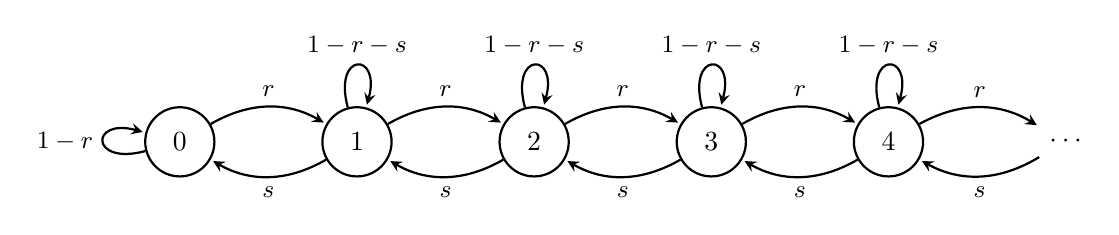
\begin{tikzpicture}[->,>=stealth,shorten >=1pt,auto,node distance=2.25cm,thick,main node/.style={scale=0.8,circle,draw,font=\sffamily\normalsize}]

            \node[state] (0) []{$0$};

            \foreach \curr [
                evaluate = \curr as \prev using {int(\curr-1)},
            ] in {1,...,4}{
                \node[state] (\curr) [right of = \prev]{$\curr$};

                \path[every node/.style={font=\sffamily\small}]
                ;
            }

            \node[] (5) [right of = 4]{$\cdots$};

            \foreach \curr [
                evaluate = \curr as \next using {int(\curr+1)}
            ] in {1,...,4}{
                \path[every node/.style={font=\sffamily\small}]
                    (\curr) edge[bend left] node{$r$} (\next)
                    (\next) edge[bend left] node{$s$} (\curr)
                    (\curr) edge[loop above] node{$1-r-s$} (\curr)
                ;   
            }

            \path[every node/.style={font=\sffamily\small}]
                (0) edge[loop left] node{$1-r$} (0)
                (0) edge[bend left] node{$r$} (1)
                (1) edge[bend left] node{$s$} (0)
            ;   

        \end{tikzpicture}
    \end{figure}

    Assuming the limiting probability exists, we consider the following stationary equations:
    \[\soe{rlcl}{
        \pi_0 &= (1-r)\pi_0 + s\pi_1 \\
        \pi_i &= r \pi_{i-1} + (1-r-s) \pi_i + s\pi_{i+1} & \qquad & \forall i > 0\\
        \sum\limits_{i = 0}^{+\infty} \pi_i &= 1
    }\]
    
    \textbf{Claim}: $\forall i > 0$ it holds that $\pi_i = \frac{r}{s} \pi_{i-1}$.

    \begin{proof}[Proof of the claim.]
        We prove by induction that forall $i > 0$ it holds that $\pi_i = \frac{r}{s} \pi_{i-1}$. By simplifying the first stationary equation, we get that $\pi_1 = \frac{r}{s} \pi_0$, proving the base case. Assuming the equality holds for $i$, we prove that the $i$-th equation implies the equality for $i+1$. In particular, we observe that $r \pi_{i-1} = s \pi_i$ is implied by the inductive hypothesis. Therefore, by substituting this in the $i$-th equation we get that:
        \[\pi_i = s \pi_i + (1-r-s) \pi_i + s\pi_{i+1} \implies \pi_{i+1} = \frac{r}{s} \pi_i \]
    \end{proof}

    Through the claim we get that $\pi_i = \rho^i \pi_0$ holds $\forall i \in \N$, where $\rho = \frac{r}{s}$. By substituting this result in the last stationary equation, we get that:
    \[1 = \sum\limits_{i = 0}^{+\infty} \rho^i \pi_0 = \pi_0 \sum\limits_{i = 0}^{+\infty} \rho^i = \pi_0 \cdot \frac{1}{1-\rho}\]

    where the last step is due to the closed form of the geometric series, concluding that $\pi_0 = 1-\rho$ and thus that $\pi_i = \rho^i(1-\rho)$ holds for all $i \in \N$ Finally, we compute $\Exp[N]$ using the definition of expected value:
    \[\Exp[N] = \sum_{i = 0}^{+\infty} i \Pr[N = i] = \sum_{i = 0}^{+\infty} i \pi_i = \sum_{i = 0}^{+\infty} i  \rho^i(1-\rho) = \rho \sum_{i = 0}^{+\infty} i  \rho^{i-1}(1-\rho) = \rho \frac{1}{1-\rho}\]

    where the last step is due to the closed form of the expected value of a geometric random variable, concluding that $\Exp[N] = \frac{\rho}{1-\rho}$. Similarly, we compute $\Exp[N^{\text{server}}]$ as:
    \[\Exp[N^{\text{server}}] = 0 \cdot \Pr[N^{\text{server}} = 0] + 1 \cdot \Pr[N^{\text{server}} \neq 0] = (1-\pi_0) = \rho\]

    and $\Exp[N^{\text{queue}}]$ through the previous values:
    \[\Exp[N^{\text{server}}] = \Exp[N] - \Exp[N^{\text{server}}] = \frac{\rho}{1-\rho} - \rho = \frac{\rho^2}{1-\rho}\]

    \begin{framedprob}{}
        We define a threshold queue with parameter $T$ as follows. When the number of jobs is less than $T$, the number of jobs decreases by 1 with probability $0.4$ and increases by 1 with probability $0.6$ at each time step. When the number of jobs increases to $T$ or more, the reverse is true: the number of jobs increases by 1 with probability $0.4$ and decreases by 1 with probability $0.6$.
        
        Assuming that the limiting probabilities exist, use the stationary equations to derive the limiting probability distribution as a function of $T$, for arbitrary threshold $T$.
    \end{framedprob}

    \textit{Solution:}

    We start by drawing the DTMC describing the problem.

    \begin{figure}[H]
        \centering

        \resizebox{1\textwidth}{!}{
            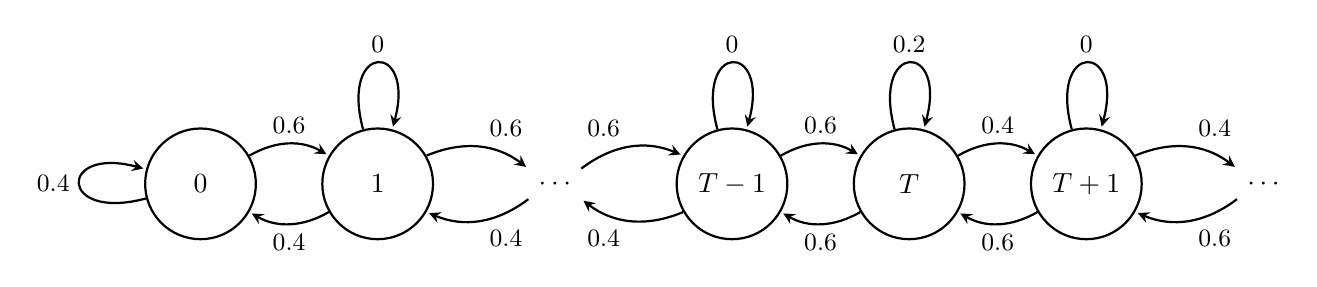
\begin{tikzpicture}[->,>=stealth,shorten >=1pt,auto,node distance=2.25cm,thick,main node/.style={scale=0.8, circle,draw,font=\sffamily\normalsize}]

                \node[state, minimum size = 40] (0) []{$0$};
                \node[state, minimum size = 40] (1) [right of = 0]{$1$};
                \node[]      (x) [right of = 1]{$\cdots$};
                \node[state, minimum size = 40] (2) [right of = x]{$T-1$};
                \node[state, minimum size = 40] (3) [right of = 2]{$T$};
                \node[state, minimum size = 40] (4) [right of = 3]{$T+1$};
                \node[]      (y) [right of = 4]{$\cdots$};

                \path[every node/.style={font=\sffamily\small}]
                    (0) edge[loop left] node{$0.4$} (0)
                    (0) edge[bend left] node{$0.6$} (1)

                    (1) edge[loop above] node{$0$} (1)
                    (1) edge[bend left] node{$0.6$} (x)
                    (1) edge[bend left] node{$0.4$} (0)

                    (x) edge[bend left] node{$0.6$} (2)
                    (x) edge[bend left] node{$0.4$} (1)

                    (2) edge[loop above] node{$0$} (2)
                    (2) edge[bend left] node{$0.6$} (3)
                    (2) edge[bend left] node{$0.4$} (x)

                    (3) edge[loop above] node{$0.2$} (3)
                    (3) edge[bend left] node{$0.4$} (4)
                    (3) edge[bend left] node{$0.6$} (2)

                    (4) edge[loop above] node{$0$} (4)
                    (4) edge[bend left] node{$0.4$} (y)
                    (4) edge[bend left] node{$0.6$} (3)
                    
                    (y) edge[bend left] node{$0.6$} (4)
                ;
            \end{tikzpicture}
        }
    \end{figure}

    Assuming the limiting probability exists, we apply the barrier technique of each pair of adjacent states. We observe that for the first $T$ states it holds that $0.6 \cdot \pi_{i-1} = 0.4 \cdot \pi_{i}$, while for the other states it holds that $0.4 \cdot \pi_{j-1} = 0.6 \cdot \pi_{j}$. Therefore, we get the following system:
    \[\soe{rlcl}{
        \pi_i &= \frac{3}{2} \pi_{i-1} & \qquad & \forall i \in \{1, \ldots, T\} \\
        \pi_j &= \frac{2}{3} \pi_{j-1} & \qquad & \forall j \in \N-\{1, \ldots, T\} \\
        \sum\limits_{i = 0}^{+\infty} \pi_i &= 1
    }\]

    By unrolling the recursive equations, we get that:
    \[\pi_k = \soe{ll}{
        \rbk{\dfrac{3}{2}}^k \pi_0 & \text{if } k \leq T \\
        \rbk{\dfrac{2}{3}}^{k-T} \rbk{\dfrac{3}{2}}^T \pi_0 & \text{if } k > T \\
    }\]

    Using the last equation, through algebraic manipulation we get that:
    \[\begin{split}
        1 &= \sum_{i = 0}^{+\infty} \pi_i\\
        &= \sum_{i = 0}^{T} \pi_i + \sum_{j = T+1}^{+\infty} \pi_j \\
        &= \sum_{i = 0}^{T} \rbk{\dfrac{3}{2}}^i \pi_0 + \sum_{j = T+1}^{+\infty} \rbk{\dfrac{2}{3}}^{j-T} \rbk{\dfrac{3}{2}}^T \pi_0 \\
        &= \pi_0 \rbk{\sum_{i = 0}^{T} \rbk{\dfrac{3}{2}}^i  + \rbk{\dfrac{3}{2}}^T \sum_{j = T+1}^{+\infty} \rbk{\dfrac{2}{3}}^{j-T}} \\
        &= \pi_0 \rbk{\frac{1-\rbk{\frac{3}{2}}^{T+1}}{1-\frac{3}{2}} + \rbk{\dfrac{3}{2}}^T \sum_{h = 0}^{+\infty} \rbk{\dfrac{2}{3}}^{h+1}} \\
        &= \pi_0 \rbk{\frac{1-\rbk{\frac{3}{2}}^{T+1}}{1-\frac{3}{2}} + \rbk{\dfrac{3}{2}}^{T-1} \sum_{h = 0}^{+\infty} \rbk{\dfrac{2}{3}}^{h}} \\
        &= \pi_0 \rbk{\frac{1-\rbk{\frac{3}{2}}^{T+1}}{1-\frac{3}{2}} + \rbk{\dfrac{3}{2}}^{T-1} \cdot \frac{1}{1-\frac{2}{3}}} \\
    \end{split}\]

    By letting $\rho = \frac{2}{3}$, we conclude that:
    \[\pi_0 = \rbk{\frac{1-\rho^{-(T+1)}}{1-\rho^{-1}} + \rho^{-(T-1)} \cdot \frac{1}{1-\rho}}^{-1}\]

    and thus that:
    \[\pi_k = \soe{ll}{
        \rho^{-k} \rbk{\frac{1-\rho^{-(T+1)}}{1-\rho^{-1}} + \rho^{-(T-1)} \cdot \frac{1}{1-\rho}}^{-1} & \text{if } k \leq T \\
        \rho^{k-2T} \rbk{\frac{1-\rho^{-(T+1)}}{1-\rho^{-1}} + \rho^{-(T-1)} \cdot \frac{1}{1-\rho}}^{-1} & \text{if } k > T \\
    }\]

    \chapter{Analysis of continuous-time systems}

    \section{The Poisson arrival process}

    Before transitioning from discrete-time Markov chains to continuous-time Markov chains in order to use them as a tool to analyze real-world systems, we have to give make some assumptions that are good enough to describe real world systems. In particular, we'll define the so called \textbf{Poisson arrival process}.

    Informally, we recall that Poisson distributions are used to describe a the number of successes in a stochastic process whose successes happen very rarely and independently. More formally, we recall that each Poisson variable $X \sim \mathrm{Poiss}(\lambda)$ corresponds to a binomial random variable $X' \sim \mathrm{Bin}(n,p)$ where $\lambda = np, n \to +\infty$ and $p \to 0$.

    We recall that binomial distributions represent the number of successes in a Bernoulli process, i.e. a sequence $X_1, \ldots, X_n$ of i.i.d. Bernoulli variables. In Bernoulli processes, the arrivals can occur only at positive integer multiples of some given increment size (often taken to be 1). It's easy to see that such process could also be characterized by the sequence $T_1, T_2, \ldots$ of \textbf{interarrival times}, where $T_i$ represents the number of failures (i.e. non-arrivals) between the $(i-1)$-th success and the $i$-th success (i.e. the $i$-th arrival). In particular, we notice that these interarrival times are geometrically distributed i.i.d. random variables: by definition, the geometric distribution represents the number of failures before a success.

    A Poisson arrival process is, in many ways, is the continuous-time version of the Bernoulli process, resulting in a simple and widely used stochastic process for modeling the times at which arrivals enter a system. Before formally defining Poisson arrival processes, we need to state some definitions.

    \begin{frameddefn}{Event sequence}
        An event sequence is a continuous time stochastic process described by a function $N : \R^+ \to \N$ such that $N(t)$ is the number of events that occurred up to time $t$.
    \end{frameddefn}

    \begin{figure}[H]
        \centering
        \includegraphics[scale=0.9]{images/poiss_arr.png}
        \caption{An event sequence where $N(t) = 4$.}
    \end{figure}

    We say that a sequence of events has \textbf{independent incrementals} if for all $t_0, \ldots, t_n$, with $n \in \N$, the random variables $X_1, \ldots, X_n$, defined as $X_i = N(t_i) - N(t_{i-1})$ for all $i \in [n]$, are all independent.
    
    Moreover, we say that a sequence of events has \textbf{stationary increments} if forall $t \in \R^+$ it holds that the random variable $X_{t,s}$, defined as $X_{t,s} = N(t-s)-N(s)$, has the same distribution for all $s \in \R^+$.

    \begin{frameddefn}{Poisson arrival process}
        A poisson arrival process with rate $\lambda$ is an event sequence such that:
        \begin{itemize}
            \item $N(0) = 0$
            \item The sequence has independent increments
            \item The number of events in any interval of length $t$ is Poisson distributed with parameter $t\lambda$. In other words, for all $t,s \in \R^+$ it holds that:
            \[\Pr[N(t+s) - N(s) = k] = \frac{e^{-\lambda t}(\lambda t)^k}{k!}\]
            with $k \in \N$.
        \end{itemize}
    \end{frameddefn}

    We observe that the third condition is just a specific case of stationary increments. Observe that the assumption of stationary and independent increments is equivalent to asserting that, at any point in time, the process probabilistically restarts itself: the process from any point onward is independent of all that occurred previously (by independent increments) and also has the same distribution as the original process (by stationary increments). In other words, the interarrival times $T_1, T_2, \ldots$ of a Poisson process are \textbf{memoryless}.

    We recall that a random variable $X$ is said to be \textit{memoryless} when:
    \[\Pr[X > t+s \mid X> s] = \Pr[X > s]\]
    
    Now, we also recall that there are only two random variables with this property: the geometric distribution (in the discrete case) and the exponential distribution (in the continuous case). Since we're in a continuous time process, we conclude that interarrival times must be exponentially distributed. In fact, we observe that the cumulative distribution function (CDF) $F_{T_i}$ for each $i \in [n]$ is equal to:
    \[\begin{split}
        F_{T_i}(t) &= \Pr[T_i \leq t] \\
        &= 1-\Pr[T_i > t] \\
        &= 1-\Pr[N(t+T_{i-1})-N(T_{i-1}) = 0] \\
        &= 1- e^{-\lambda t}\\
    \end{split}\]
    
    which is exactly the CDF of an exponential distribution. Of course, the converse can also be proven, but it requires a way more formal proof. 

    \begin{framedthm}{Poisson arrival process (2° def.)}
        A Poisson process with rate $\lambda$ is a sequence of events such that $N(0) = 0$ and the interarrival times $T_1, T_2, \ldots$ are i.i.d. exponential random variables of parameter $\lambda$.
    \end{framedthm}

    \begin{proof}
        Omitted.
    \end{proof}

    The Poisson process is the most widely used model for arrivals into a system for two main reasons. First, the Markovian properties of the Poisson process make it analytically tractable. Second,  many phenomena that are the aggregate effect of a large number of individuals behave in a Poisson fashion. For instance, in communications networks, such as the telephone system, it is a good model for the sequence of times at which telephone calls are originated. Although the calls of a single user do not look like a Poisson process, the aggregate over many users does.

    \section{Continuous-time Markov Chains}

    After defining the Poisson process, we're ready to jump to the continuous analogous, i.e. \textbf{continuous-time Markov chains (CTMC)}. We start by giving a formal definition, similar to the discrete case.

    \begin{frameddefn}{Continuous-time Markov Chain}
        We define a continuous-time Markov chain (CTMC) as an continuous stochastic process $\{X(t) \mid t \geq 0\}$ such that:
        \begin{itemize}
            \item $\mathcal{I}$ is the state space
            \item $\forall t \geq 0$, $X(t)$ is the random variable ranging over $\mathcal{I}$ and describing the state of the system at (continuous) time step $t$.
            \item The Markovian property holds for each state, meaning that $\forall t,s \in \N$, $\forall j, i \in \mathcal{I}$ and $\forall x : \R^+ \to \mathcal{I}$ it holds that:
            \[\Pr[X(t+s) = j \mid X(s) = i, X(u) = x(u), 0 \leq u \leq s] = \Pr[X(t+s) = j \mid X(s) = i]\]
        \end{itemize}
    \end{frameddefn}
    
    It's easy to see that through this definition we cannot easily establish a graphical model to represent CTMC due to the absence of discrete time. We'll build an intuition through the following discussion.
    
    Let $\tau_i$ be the time until the CTMC leaves state $i$, given that the CTMC is currently in state $i$. By the Markovian and stationary properties of the CTMC, the probability that the CTMC leaves state $i$ in the next $t$ seconds is independent of how long the CTMC has already been in state $i$. In other words, we have that:
    \[\Pr[\tau_i > t+s \mid \tau_i > s] = \Pr[\tau_i > t]\]
    which corresponds to the \textit{continuous memorylessness property}. Therefore, this argument allows us to conclude that a CTMC is a continuous stochastic process with the property that every time it enters state $i$, the following hold:
    \begin{enumerate}
        \item The amount of time $\tau_i$ that the process spends in state $i$ before making a transition is exponentially distributed with some rate $\nu_i$, i.e. $\tau_i \sim \mathrm{Exp}(\nu_i)$.
        \item When the process leaves state $i$, it will next enter state $j$ with some probability $p_{i,j}$ independent of the time spent at state $i$, where $\sum_{j \in \mathcal{I}} p_{i,j} = 1$
    \end{enumerate}

    \begin{figure}[H]
        \centering
        \includegraphics[scale=0.85]{images/ctmc_1.png}
        \caption{First way to view CTMCs.}
    \end{figure}

    Observe that $p_{ij}$, the probability that when we leave $i$ we next go to state $j$, is a constant: it is independent of time $t$ (by stationarity) and it is independent of the time $\tau_i$ spent in state $i$ (by Markovian property). Now, consider the moment just before we leave state $i$. At this moment, the time we have spent in state $i$ is irrelevant (again, by Markovian property). All that is relevant is that we are at state $i$ at this moment $s$. The particular time $s$ is irrelevant as well (by stationarity). 

    This gives us another way to view CTMCs. Let $X_j  \sim \mathrm{Exp}(\nu_i p_{ij})$ represent the time to transition from $i$ to $j$, for all $ i \neq j$. Let $\tau_i = \min_{j \in \mathcal{I}}(X_j)$ be the time until the CTMCs leaves state $i$. Then, the next state $m$ is given by $m = \argmin_{j \in \mathcal{I}} (X_j)$, i.e. the state that minimizes the time waited until the CTMC leaves state $i$.

    \begin{figure}[H]
        \centering
        \includegraphics[scale=0.85]{images/ctmc_2.png}
        \caption{Second way to view CTMCs.}
    \end{figure}

    We won't formally prove the equivalence between the two views, as the above discussion suffices. Now, conside the following open system with continuous arrival and service rates.
    \begin{figure}[H]
        \centering
        \includegraphics[scale=0.9]{images/ctmc_3.png}
        \caption{An open system with continuous arrival and service rates.}
    \end{figure}

    Using the second way to view CTMCs, we can model the problem through the following diagram.

    \begin{figure}[H]
        \centering

        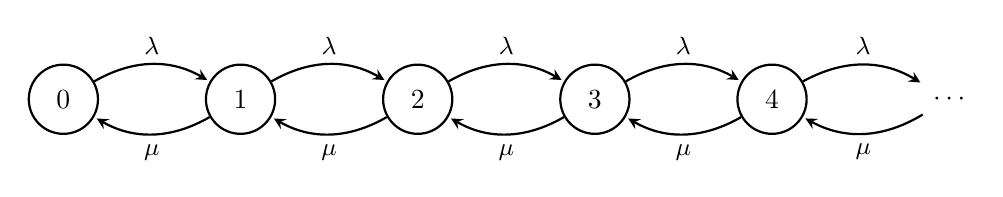
\begin{tikzpicture}[->,>=stealth,shorten >=1pt,auto,node distance=2.25cm,thick,main node/.style={scale=0.8,circle,draw,font=\sffamily\normalsize}]

            \node[state] (0) []{$0$};

            \foreach \curr [
                evaluate = \curr as \prev using {int(\curr-1)},
            ] in {1,...,4}{
                \node[state] (\curr) [right of = \prev]{$\curr$};
            }

            \node[] (5) [right of = 4]{$\cdots$};

            \foreach \curr [
                evaluate = \curr as \next using {int(\curr+1)},
            ] in {1,...,4}{
                \path[every node/.style={font=\sffamily\small}]
                    (\curr) edge[bend left] node{$\lambda$} (\next)
                    (\next) edge[bend left] node{$\mu$} (\curr)
                ;   
            }

            \path[every node/.style={font=\sffamily\small}]
                (0) edge[bend left] node{$\lambda$} (1)
                (1) edge[bend left] node{$\mu$} (0)
            ;   

        \end{tikzpicture}

        \caption{The continuous-time Markov chain of the previous example.}
    \end{figure}

    In particular, we observe that loops are not required: in this context, transitions represent the time waited before the state changes, not the probability of changing state! A natural question rises: do we require a brand new method to solve CTMCs? The answer, to some extent, is no: the idea is to \textbf{uniformize and discretize time} in order to study continuous-time processes using the descrete-time methods that we have already learned.
    
    To achieve this, we can define a very small time interval $\delta$, called \textit{observation time}, and observe the state assumed by the continuous-time process every $\delta$ seconds. Then, given the \textit{observation rate} $\Delta = 1/\delta$, we get that:
    \[p_{\text{increase}} = \frac{\lambda}{\Delta} \qquad\quad p_{\text{decrease}} = \frac{\mu}{\Delta}\]

    We notice that in order for this idea to make sense, the observation rate $\Delta$ must be many times higher than any rate of the CTMC, i.e. $\Delta >> \lambda, \mu$. After defining such probabilities, we can define a DTMC \curlyquotes{equivalent} to the origianl CTMC. This DTMC is referred to as \textbf{Embedded Discrete-time Markov chain (EDTMC)}.

    \begin{figure}[H]
        \centering

        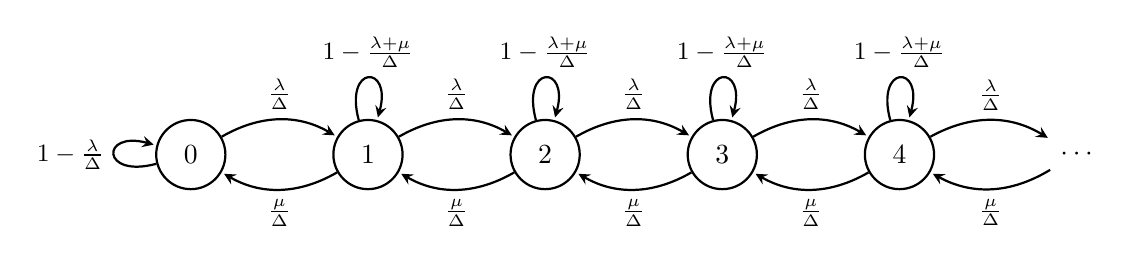
\begin{tikzpicture}[->,>=stealth,shorten >=1pt,auto,node distance=2.25cm,thick,main node/.style={scale=0.8,circle,draw,font=\sffamily\normalsize}]

            \node[state] (0) []{$0$};

            \foreach \curr [
                evaluate = \curr as \prev using {int(\curr-1)},
            ] in {1,...,4}{
                \node[state] (\curr) [right of = \prev]{$\curr$};
            }

            \node[] (5) [right of = 4]{$\cdots$};

            \foreach \curr [
                evaluate = \curr as \next using {int(\curr+1)},
            ] in {1,...,4}{
                \path[every node/.style={font=\sffamily\small}]
                    (\curr) edge[loop above] node{$1-\frac{\lambda + \mu}{\Delta}$} (\curr)
                    (\curr) edge[bend left] node{$\frac{\lambda}{\Delta}$} (\next)
                    (\next) edge[bend left] node{$\frac{\mu}{\Delta}$} (\curr)
                ;   
            }

            \path[every node/.style={font=\sffamily\small}]
                (0) edge[loop left] node{$1-\frac{\lambda}{\Delta}$} (0)
                (0) edge[bend left] node{$\frac{\lambda}{\Delta}$} (1)
                (1) edge[bend left] node{$\frac{\mu}{\Delta}$} (0)
            ;   

        \end{tikzpicture}

        \caption{The embedded discrete-time Markov chain of the previous example.}
    \end{figure}

    Now, we can apply the barrier technique to compute the limiting distribution $\pi$ of the EDTMC. In particular, we observe that for any pair of adjacent states we have that:
    \[\frac{\lambda}{\Delta} \pi_{i-1} = \frac{\mu}{\Delta} \pi_{i} \implies \lambda \pi_{i-1} = \mu \pi_{i}\]
    giving us the following system of stationary equations:
    \[\soe{rlcl}{
        \lambda \pi_{i-1} &= \mu \pi_{i} & \qquad & \forall i \in \N-\{0\} \\
        \sum_{i = 0}^{+\infty} \pi_i &= 1
    }\]

    In other words, the value chosen for $\Delta$ (or $\delta$) doesn't influence the solutions! This is the fundamental idea that allows us to solve CTMCs by directly applying the \textbf{barrier technique} to the CTMC, without passing through the EDTMC.

    \begin{figure}[H]
        \centering

        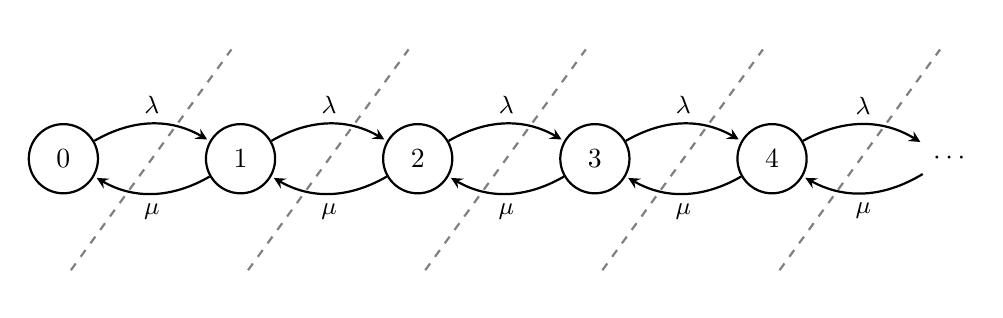
\begin{tikzpicture}[->,>=stealth,shorten >=1pt,auto,node distance=2.25cm,thick,main node/.style={scale=0.8,circle,draw,font=\sffamily\normalsize}]

            \node[state] (0) []{$0$};

            \foreach \curr [
                evaluate = \curr as \prev using {int(\curr-1)},
            ] in {1,...,4}{
                \node[state] (\curr) [right of = \prev]{$\curr$};

                \node[] (x\prev) [below of = \prev, yshift=20]{};
                \node[] (y\curr) [above of = \curr, yshift=-20]{};

                \path[-, every node/.style={font=\sffamily\small}]
                    (x\prev) edge[dashed, color = gray] (y\curr)
                ;
            }

            \node[] (5) [right of = 4]{$\cdots$};

            \node[] (x5) [below of = 4, yshift=20]{};
            \node[] (y5) [above of = 5, yshift=-20]{};

            \path[-, every node/.style={font=\sffamily\small}]
                (x5) edge[dashed, color = gray] (y5)
            ;

            \foreach \curr [
                evaluate = \curr as \next using {int(\curr+1)},
            ] in {1,...,4}{
                \path[every node/.style={font=\sffamily\small}]
                    (\curr) edge[bend left] node{$\lambda$} (\next)
                    (\next) edge[bend left] node{$\mu$} (\curr)
                ;   
            }

            \path[every node/.style={font=\sffamily\small}]
                (0) edge[bend left] node{$\lambda$} (1)
                (1) edge[bend left] node{$\mu$} (0)
            ;   

        \end{tikzpicture}

        \caption{Application of the barrier technique to a continuous-time Markov chain.}
    \end{figure}

    \section{Kendall's model}

    Up until now, we have strictly focused on devices formed of an infinite queue and server. Now, we'll discuss devices in a more general way. First of all, we introduce a \textit{notation} that will allow us to talk about devices in a more coincise way. In particular, we'll use \textnormal{Kendall's notation}, that is the notation $M/M/k/M_Q$ where:
    \begin{itemize}
        \item The first $M$ stands for \textit{memoryless arrivals}
        \item The second $M$ stands for \textit{memoryless departures}
        \item The parameter $k$ stands for the number of servers connected to unique queue
        \item The parameter $k$ stands for the size of the unique queue
    \end{itemize}  

\end{document}
